\documentclass[a4paper, french, 12pt]{article}  % DŽclare la classe du document.
% Il existe 5 classes sous LaTeX : article, book, report, letter et slides 
% Les options de classe sont entre crochets et permettent de faire des choix d'ordre gŽnŽral :
% - dŽfinir la taille de base des caractres avec 10pt, 11pt, 12pt, les commandes d'agrandissement 
% ou de rŽduction de la tailles des caractres ( \small \large ) se feront alors par rapport ˆ cette base
% - dŽfinir la taille du papier:  a4paper,  a5paper, b5paper, executivepaper, legalpaper ou letterpaper
% Utiliser a4paper ds que la papier utilisŽ est de ce format c'est ˆ dire ... tout le temps ;-)
% - utiliser des options de mise en page : 
%       ->   landscape passe en mode paysage pour l'ensemble du doccument
%       ->   onecolumn  option par dŽfaut, le texte sera sur une seule colonne 
%       ->   twocolumn   pour un doccument sur deux colonnes, des rŽglages sont possibles (cf doc & net)
%       ->   oneside toutes les pages seront traitŽs identiquement, par dŽfaut avec la classe article
%       ->   twoside  mise en page diffŽrentes pour les pages pairs et impairs par dŽfaut avec book
%       ->   openright et openany  pour gŽrer le commencement des chapitres dans la classe book
%       ->   titlepage et notitlepage indique si une nouvelle page doit tre commencŽe aprs le titre du document.
 
% \usepackage permet de dŽclarer un module qui sera pris en compte dans la suite. 
% Les modules permettent d'Žtendre les fonctionnalitŽ de LaTeX

%%%%Caracteres reserves%%%%%%%%%%%
%Pour les obtenir on les fait précéder d'un \
% { s'obtient avec \{
% } s'obtient avec \}
% % s'obtient avec \% 
% $ s'obtient avec \$
% & s'obtient avec \&
% # s'obtient avec \#
% _ s'obtient avec \_
% ^ s'obtient avec \^{}
% \ s'obtient avec \textbackslash{} car \\ est une commande
%Les caractères [ et ] ne sont pas réservés et s'obtiennent directement
%\[ et \] delimitent une environnement mathematique
%%%%%%%%%%%%%%%%%%%%%%%%%%%%%%%%%%%%%%%%%%%


%%%%%Polices%%%
%La police employee par defaut par Latex s'appelle Computer Modern

%%%Changement de style de police%%

%Police par defaut {\normalfont ...} c'est une bascule

%Trois familles 
%Romaine par defaut
%sans serif \textsf{..} ou {\sffamily ....}
%typewriter \texttt{..} ou {\ttfamily ....}

%Quatre formes
%droite par defaut
%italique \textit{..} ou {\itshape ....}
%penchee \textsl{..} ou {\slshape ....}
%petites capitales  \textsc{..} ou {\scshape ....}

%Deux series
%normale par defaut
%grasse \textbf{..} ou {\bfseries ....}


%%Taille%%
%Toutes les commandes suivantes sont des bascules a utiliser entre accolades
%{\tiny petit mot}
%Dans l'ordre croissant
%\tiny
%\scriptsize
%\footnotesize
%\small
%\normalsize
%\large
%\Large
%\LARGE
%\huge
%\Huge

%%%%%%%%%%%%%%%%%%%%%%%%%

%%%%%Justification%%%%%
%Alignement a droite
%\begin{flushright}
%{\raggedleft texte \par} ne pas oublier \par
%\leftline{texte}
%\filleft pour formater un titre 

%Alignement a gauche
%\begin{flushleft}
%{\raggedright texte \par} ne pas oublier \par
%\rightline{texte}
%\filright pour formater un titre 


%Centrage
%\begin{center}
%{\centering texte \par} ne pas oublier \par
%\centerline{texte}
%\filcenter pour formater un titre 
%%%%%%%%%%%%%%%%%%%%%%%%%%%%%%%%%%%%%%%%%%%

%%%%%%Espaces%%%%%%%%%%%%%%%%%%%%%


%%Espaces verticaux%%%
%\vskip 2cm  (argument eventuellement negatif), l'espace est ignore s'il coincide avec un saut de page
%\vspace*{2cm} (argument eventuellement negatif), l'espace n'est pas ignore s'il coincide avec un saut de page
%\vspace{2cm} est synonyme de \vskip 2cm 

%%Espaces horizontaux%%%%

%\hskip equivalent a \vskip
%\hspace{?} et \hspace*{?}
%Le cadratin est un espace horizontal egal a la taille de la police utilisee
%\thinspace espace d'un sixieme de cadratin
%\enskip pour un demi-cadratin
%\quad pour un cdratin
%\qquad pour deux cadratins

%%%%%%%%%%%%%%%%%%%%%%%%%%%%%%%%%%%%

%Le moteur eTeX est aujourd'hui utilisé par toutes les distributions (MikTeX, TeXlive) à la place de l'ancien TeX (en fait, c'est plutôt PDFTeX, le successeur de eTeX, qui est utilisé ; contrairement à ce que son nom indique, il peut produire du dvi). Le fait d'utiliser le moteur eTeX au lieu de TeX donne accès à des choses en plus (par exemple à \middle pour aller avec \left et \right, mais aussi à des commandes bien pratiques comme \numexpr, \dimexpr, \detokenize, etc. ainsi qu'à des ressources supplémentaires, comme plus de compteurs disponibles).

%Lorsqu'on utilise le moteur eTeX, certaines de ces fonctionnalités sont automatiquement accessibles (c'est le cas de \middle, \numexpr, etc.), mais pas d'autres (c'est le cas des compteurs supplémentaires). Pour activer ces fonctionnalités manquantes, on peut charger le package etex.sty. Ainsi, l'utilisation d'etex.sty est une solution courante au problème d'avoir trop de compteurs définis (c'est le cas si on charge ensemble trop de packages du type tikz, pstricks, xymatrix, ...)

\usepackage{etex}

%%%%%%%%%%%%Encodage du fichier source %%%%%%%%%%%
\usepackage[T1]{fontenc}
\usepackage[utf8]{inputenc}


%%%%%%%%%%%%%%%Francisation%%%%%%%%%%%%%%
\usepackage[french]{babel}
\frenchbsetup{StandardLists=true}
%%%%%%%%%%%%%%%%%%%%%%%%%%%%%%%%%%%%%%%%%

%%%%%%%%%%%%Mise en page, Reglages genrraux%%%%%%%

%\title{il n'existe pas de plus grand nombre premier}
%\author[Euclide \thanks{Merci Aristote}}
%\date{12 juin $-260$}  Par défaut Latex insère la date du jour
%puis écrire après \begin{document} la commande \maketitle


\usepackage[a4paper,headheight=35 pt, headsep=15pt,top=20 pt,hmargin=1 cm,bottom=20 pt,includeheadfoot]{geometry}
%\usepackage[a4paper,hmargin=1 cm,bottom=2cm,top=2cm,headheight=15pt]{geometry}      
%top est la marge supérieure entre le haut de body et le bord supérieur de la feuille
% \usepackage[left= 4cm,right = 3cm,top= 2cm, bottom=2cm]{geometry} pour le réglage des marges 
% \usepackage[top= 17mm,textheight=23cm,heightrounded,left=25mm,textwidth=16cm] {geometry} pour fixer la hauteur,  la largeur  du texte. heightrounded, autorise le package à arrondir la hauteur textheight à un nombre entier de lignes pour éviter des problèmes de remplissage vertical underfull vbox 


\usepackage{setspace}  % pour le réglage de l'interligne
%Bascule \doublespacing  ou environnement {doublespace}
%Bascule \onehalfspacing  ou environnement {onehalfspace}
%Bascule \singlespacing  ou environnement {singlespace}
% ou encore \renewcommand{\baselinestretch}{n} ou encore l'environnement spacing{n}

%%Package fullpage
%\usepackage[cm]{fullpage}
%where possible options for fullpage are
%in (default) sets the margins to one inch;
%cm sets the margins to 1.5 cm (one centimeter is really too
%little);
%plain (default) selects the plain page style, i.e., with no head-
%ers but only a footer;
%empty for neither headers nor footers;
%headings for both header and footers;
%myheadings also for both headers and footers.
%For the last 4 options, the corresponding \pagestyle declaration is exe-
%cuted, so that it is not necessary to give it again.


%%Pour la numerotation des bas de pages avec le compteur lastpage%%%
\usepackage{lastpage}

%%%%Pour afficher certaines pages au format paysage%%
\usepackage{lscape}
%\begin{landscape}

%%%Plusieurs colonnes
\usepackage{multicol}
%\begin{multicols}[titre]{nb colonnes}
\setlength{\columnseprule}{0.25pt}


%%%%%Références, Notes de bas de pages ou de marges%%%%%%%%%

%%Pour placer une note de bas de page : commande \footnote{}
%Pour placer une note dans la marge : \marginpar{}
%Pour plcaer une note dans un tableau : appel de note avec \footnotemark{} puis le texte après le tableau avec \footnotetext{texte}

%Etiquette  avec \label{nom} puis référence à l'étiquette (numéro de section le plus proche ) avec \ref{nom} ou à lap age avec \pageref{nom}
\usepackage{varioref}
%Introduit  les commandes \vref{} et \vpageref{} qui améloirent l'affichage ainsi que la commande \vpagerefrange{label1}{label2} pour faire référence à tout un bloc de pages entre deux étiquettes
\usepackage{nameref}


%%%%Présentation des titres de section%%%

%\usepackage[clearempty]{titlesec} problème avec PDFLatex ?

%Pour changer la police des titres de sectionnement, un exemple :
%\titleformat*{\section}{\sffamily}

%Pour modifier la police mais aussi la présentation :
%\titleformat{commande}[shape]{format}{label}{sep}{before}{after}
% commande est la commande de sectionnement comme \section
%shape peut etre hang (défaut),frame (encadre), display( paragraphe séparé), block (paragraphe), runin (dans le texte, wrap (comme wrapfigure), leftmargin ou rightmargin
%format est le formatage du titre complet (numéros inclus)éventuellemnt précédé de commandes à inclure avant le titre
% Ces commandes peuvent etre \titleline[r,c ou l]{texte} ou \titlerule[epaisseur] ou \titlerule*[epaisseur]{texte}
%label est la présentation du numero
%sep est l'espace entre le numero et le titre
%before est le code à exécuter avant le titre de section (numero exclu)
%after est le code à exécuter après (vide en général)

%Pour gérer l'espacement
%\titlespacing{commande}{left}{beforesep}{aftersep}[right]
%left est la marge à gauche, beforesep l'espace vertical avant etc ..


%Exemple de présentation de titre encadé :
%\titleformat{\section}[frame]{\titleline[r]{\rule{2in }{2pt}} \normalfont}{\filright\small\ SECTION \thesection\hfill}{7pt}{\LARGE \bfseries\filcenter}{}
%\section{un titre de section encadre}


%%%%%%%%%%%%%%%%%%%%%%%%%%%%%%%%%%%%%%%%%%%% 

%%%%%%%Réglages de la table des matières%%%%
\usepackage{tocvsec2}
%Définir la progondeur : \setcounter{tocdepth}{1}  :
%1 correspond aux chapitres; 2 aux sections etc ...
%Rédéfinir le nom par défaut  :
%\renewcommand{\contentsname}{Liste des chapitres}
%Modifier une entrée :
%\Chapter[titre court]{titre long}
%Ajouter une entrée :
%\addcontentsline{toc}{section}{Nom de la section qu'on veut ajouter}
%Pour exclure une entrée 
%Utiliser une commande étoilée comme \section*
%Pour ajouter  ce qu'on veut dans la table des matières comme des indications de mise n page :
%\addtocontents{toc}{\protect \pagebreak}


%%%%%%%%%%%% Packages pour le texte %%%%%%%%%%%%
\usepackage{lmodern}       %Joli fonte

\usepackage{pifont,fourier}
\usepackage[normalem]{ulem}
%\uline{} pour  un soulignement simple
%Commmandes \uuline{} pour un soulignement double
%\uwave{} pour un soulignement  avec des vagues
% \sout{} pour barrer et \xout{} pour hachurer
\usepackage{cancel} %Commande \cancel{} pour barrer en oblique
%\usepackage{soul}    %souligner
%\usepackage{lettrine} %Pour commencer un paragraphe avec une lettrine
%Package incompatible avec tabvar.tex
%\lettrine{S}{i vous souhaitez}
%\renewcommand{\LettrineFontHook}{\itshape}
%\renewcommand{\LettrineTextFont}{\sffamily}

%%%Pour des jolis boites%%%
\usepackage{fancybox}  
%Commandes \box{} \ovalbox{} \shadowbox{}
%\cornersize{}2 réglage de l'arrondi
% Dimension à régler avec \setlength{}  : \fboxsep \fboxrule  

%%% Pour faire tourner le texte %%%
\usepackage{rotating}  %\begin{turn}{-60} tourné \end{turn} pour tourner un paragraphe
						%pour tourner un texte, commande \rotatebox[origin=c]{angle}{texte}
						
%%Divers%%%%
\usepackage{eurosym}  %pour le symbole de l'euro

\usepackage{url} %pour la gestion des adresses web avec la commande \url{}

%%%%%%%%%%%

%%%%%%%%%%%%%%%Ecriture d'algorithmes Insertion de code source %%%%%%%%%%%

%%%%%Package verbatim%%%%

\usepackage{verbatim} 
%LE package verbatim améliore la présentation des verbatim
% Il  fournit un environnement {comment} pour insérerer des commentaires
%dans le fichier source sans faire précéder toutes les lignes de %

\usepackage{alltt, moreverb} 
%L'environnement verbatimboxed permet d'encadrer un texte en verbatim
% De plus les caractères spéciaux \ et { ne sont pas désactivés (mais #, $ et % le sont)
% et on peut saisir des formules mathématiques avec \( .. \) ou \[ ... \]

%%Pour améliorer envore la présentation des verbatim%%%%
\usepackage{fancyvrb}


%%Couleur
\usepackage[table]{xcolor} 


%%%%%%%%%% Nouvelles couleurs
\definecolor{rouge}{rgb}{1,0,0}
\definecolor{bleu}{rgb}{0,0,1}
\definecolor{orange}{rgb}{1.00,0.50,0.00}
\definecolor{vert}{rgb}{0,0.50,0.00}
\definecolor{marron}{rgb}{0.49,0.16,0.06}
\definecolor{mauve}{rgb}{0.42,0.24,0.77}
\definecolor{rpastel}{rgb}{1.00,0.77,0.77}
\definecolor{bpastel}{rgb}{0.70,0.86,0.93}
\definecolor{grisclair}{gray}{0.85}
\definecolor{gristclair}{gray}{0.95}
\definecolor{grisfonce}{gray}{0.4}



%%%%%%%%%%%%%%%%%%¨Puce, Listess%%%%%%%%%%%%%%
\usepackage{enumerate}
\usepackage{enumitem}
%Pour changer la puce de liste dans tout le document :
%AtBeginDocument{\renewcommand{\labelitemi}{\textbullet}}
%%%%%%%%Réglages spécifiques au document%%%%%%%%%

%\setenumerate[1]{label=\textbf{Q\arabic*)}}


%%%%%%%%%%%%Graphiques et Dessins%%%%%%%%%%%%%%

\usepackage{graphicx}		
%\rotatebox[origin=x0x1]{angle}{texte} avec xox1 parmi t (top) l (left) r (right) B (ligne de base) et b (bottomm)
%\resizebox{largeur}{hauteur}{texte} pour faire rentrer u nelement encombrant dans une boite					


\usepackage{epic,eepic}   %Capacités graphiques étendues
%\begin{picture}(0,0) permet d'insérer n'importe quoi, n'importe où sans prendre de place (utilie pour annoter une figure en eps)
%Une autre technique est \makebox[0cm][alignement]{texte}
%Exemple:
%\includegraphics[scale=1]{singe.eps}
%\begin{picture}(0,0)
%\put(-27,10){$\sqrt[3]{8}$}
%\end{picture}



%%%%%%%%%%PSTricks%%%%%%%%%%%%

\usepackage{pstricks,pst-plot,pst-text,pst-tree,pst-eps,pst-fill,pst-node,pst-math,pstricks-add,pst-xkey,pst-eucl}


%%%%%%%Tikz%%%%%%%%%%%%%%%
\usepackage{pgf,tikz,tkz-tab}
% Pour les tableaux de signes ou de variations avec tkz-tab voir https://zestedesavoir.com/tutoriels/439/des-tableaux-de-variations-et-de-signes-avec-latex/#1-13389_tikz-un-package-qui-en-a-dans-le-ventre
\usetikzlibrary{arrows}
\usetikzlibrary{shapes.geometric}
\usetikzlibrary{petri}
\usetikzlibrary{decorations}
\usetikzlibrary{arrows}



%%%%%%%%%%%%%%%%%%%%%%%%%%%%%%%%%%%%%%%%
%%%%%%%%%%%Commandes Tikz Perso%%%%%%%%%%%%%%%

% Définition des nouvelles options xmin, xmax, ymin, ymax
% Valeurs par défaut : -3, 3, -3, 3
\tikzset{
xmin/.store in=\xmin, xmin/.default=-3, xmin=-3,
xmax/.store in=\xmax, xmax/.default=3, xmax=3,
ymin/.store in=\ymin, ymin/.default=-3, ymin=-3,
ymax/.store in=\ymax, ymax/.default=3, ymax=3,
}
% Commande qui trace la grille entre (xmin,ymin) et (xmax,ymax)
\newcommand {\grille}[2]
{\draw[help lines,black, thick] (\xmin,\ymin) grid[xstep=#1, ystep=#2] (\xmax,\ymax);}
% Commande \axes
\newcommand {\axes} {
\draw[->,very thick] (\xmin,0) -- (\xmax,0);
\draw[->,very thick] (0,\ymin) -- (0,\ymax);
\draw (0.95*\xmax, 0) node[above] {$x$};
\draw (0, 0.95*\ymax) node[left] {$y$};
}
% Commande qui limite l?affichage à (xmin,ymin) et (xmax,ymax)
\newcommand {\fenetre}
{\clip (\xmin,\ymin) rectangle (\xmax,\ymax);}

%Exemple d'utilisation

%\begin{center}
%\begin{tikzpicture} [xmin=-2,xmax=2,ymin=0,ymax=5]
%\grille{1} \axes \fenetre
%\draw plot[smooth] (\x,\x^2);
%\end{tikzpicture}
%\end{center}

%style pour la perspective cavalière française
%voir Tikz pour l'impatient page 68
\tikzset{math3d/.style=
{x= {(-0.353cm,-0.353cm)}, z={(0cm,1cm)},y={(1cm,0cm)}}}

%%%%%%%Symbole pour code calculatrice%%%%%%

%Flèche remplie pour défilement de menu

\newcommand{\flechefillright}{
\begin{tikzpicture}[scale=0.15] \fill (0,0)--(2,1)--(0,2)--cycle;
\end{tikzpicture}}

%%%%%%%%%%%%%Symboles pour calculatrice Casio%%%%
\newcommand{\execasio}{\Pisymbol{psy}{191}} %Retour chariot
\newcommand{\dispcasio}{\begin{pspicture}(.1,.1)\pspolygon*(.1,0)(.1,.1)\end{pspicture}} %Triangle « Disp »
\newcommand{\dispcasiotikz}{\begin{tikzpicture}[scale=0.2]
\fill (0,0) -- (1,0) -- (1,1) -- cycle;
\end{tikzpicture}} %Triangle « Disp »
%

%Fleche entre deux lignes, d'apres 'un bon petit' : http://forum.mathematex.net/latex-f6/fleches-entre-deux-lignes-pour-resolution-d-equation-t10283.html#p99817
\newcommand\addnode[1]{\Rnode{#1}{}}
\newcommand\linknode[3]{\ncbar[angleA=0,angleB=0,nodesep=1ex,arm=10ex,offset=-2pt]{->}{#1}{#2}\Aput{\vphantom{x}#3}}

%%%%%%%%%%%%%%%%%%%%%%%%%%%%%%%%%%%%%%%%
%%%%%%%%%%%Fin Commandes Tikz%%%%%%%%%%%%%%%


%%%%%%%%%%%%Specifiques%%%%%%%%%%%
\usepackage{wrapfig}
%pour insérer une figure à droite ou à gauche d'un texte
%\begin{wrapfigure}[nb lignes]{placement l,r,c,i(inside),o(outside)}[overhang]{width}
%ce package fonctionne mal à proximité des listes
%%%%%%%%%%%%%%%%%%%%%%%%%%%%%%%%%%%%%

%%%%%Environnements et symboles spéciaux pour faire joli%%%%%%

%%%Pour des environnements + jolis avec insertion de logo%%%%
\usepackage{xkeyval}  %indispensable pour bclogo
\usepackage[tikz]{bclogo}

\usepackage{framed}  %Le package « framed» Crée 3 nouveaux environnements, qui se comportent comme des minipage de largeur \linewidth, mais permettant en plus de se casser entre plusieurs pages.     * framed : avec un cadre autour;     * shaded : avec un fonc coloré (il faut définir la couleur shadecolor);     * leftbar : avec une barre le long du côté gauche.

%%%%%%%%%%%%%%%%%%%%%%%%%%%%%%%%%%%


%%%%%%Environnements et symbomles mathématiques%%%%

%%%Tableaux de variations %%%%%%%%%%

\usepackage{variations}

%%%%%%%%%%%AmsMaths%%%%%%
\usepackage{mathtools}        %Commandes essentielles, extension d'amsmath
\usepackage{amsfonts,amssymb}  %Principaux symboles
\usepackage{mathrsfs} %Polices calligraphiques
\usepackage{stmaryrd} %Pour les intervalles d'entiers avec \llbracket et \rrbracket
\usepackage[autolanguage, np]{numprint}
%%%%%%%%%%%%Là encore il y a de grosses différences entre le monde anglo-saxon et les francophones.Le séparateur des décimales est un point en anglais et une virgule en français. Leséparateur des milliers est une virgule en anglais et une espace insécable en français. Ilest préférable d’utiliser le package numprint (\usepackage{numprint}) qui associé àfrenchb produira la bonne typographie.
%123456789 = 123456789 \numprint{123456789} = 123 456 789  \numprint{3,1415926535897932384626} = 3,141 592 653 589 793 238 462 6  \numprint{12.34} = 12,34  En plus tu peux préciser les unités de cette façon : \numprint[kg]{12.34} = 12,34 kg ou encore \numprint[\degres C]{22} = 22°C Si tu veux utiliser le raccourci \np{} au lieu de \numprint{}, il te faut charger le package de cette façon : \usepackage[np]{numprint}
\usepackage[thmmarks,amsmath]{ntheorem}
%Pour définir un nouveau théorème :
%\newtheorem{conj}{Conjecture}[chapter] environnement con d'en tete Conjecture avec numérotation au sein d'un chapitre
%Pour rédéfinir le style d'un théorème, placer les commandes avant \newtheorem et entourer le tout d'accolades
%\theoremstyle{style} : :
% plain est le style par défaut
% break insère un saut de ligne après le titre du théorème
%margin et marginbreak sont les équivalents avec numéro dans la marge
%\theorembodyfont{\normalfont \sffamily} police du corps du théorème
%\theoremheaderfont{\scshape} police de l'en-tete (définie 1 fois pour tous les théorèmes)
%\theoremsymbol{ } symbole ajouté à la fin du théorème
%\theoremseparator{--} élément situé entre le numéro et le corps du theoreme
%\theoremprework{\rule{\linewidth}{0.4pt}} élément précédant chaque théoreme
%\theorempostwork{\dingline{71}} élément suivant chaque théoreme
%\theoremnumbering{Roman} style de numérotation
\usepackage{bbm, dsfont}   %Fonction indicatrice
\usepackage{esint,esvect}  %Flèches supplémentaires.
\usepackage{lcg}  %%%%%%%générer des nombres pseudo aléatoires%%%%


%%%%%%%%%%%Tableaux%%%%%%%%%%%
\usepackage{array}
%\usepackage{multirow} %problème redéfinit la commande \multirow{nligne}*{texte}
\usepackage{tabularx}        % Largeur totale donnée          
\usepackage{longtable}       %Sur plusieurs pages
%\usepackage{diagbox}  %Successeur de slashbox, voir Latex pour l'impatient p. 73, charge pict2e qui redefinit \arc
\usepackage{alterqcm} 
%%%Une commande de David Robert%%%%%%%
%\newcommand{\delair}[1]{\ensuremath\displaystyle\psframebox[framesep=0.15em,linestyle=none]{ \displaystyle#1}}
\newcommand{\delair}[1]{\setlength{\fboxrule}{0mm} \fbox{#1}}
%%%%%%%%%%%%%%%%%%%%%%%%%%%%%%%%%%%%%%




%%%%%%%%%%%%%%Programmation en Latex, Création de nouvelles Commandes%%%%%%%%%%%%%
\usepackage{xspace} %pour la gestion fine des espaces avec la commande \xspace
\usepackage{calc} %   pour faire des calculs avec les longueurs par exemple%%
%Commande \real{0.72} pour le reel 0,72
%\ratio{3}{4} pour le reel 0,75

\usepackage{ifthen}
%Syntaxe d'un test conditionnel : \ifthenelse{condition}{action si realisee}{action sinon}
%Commandes de test :
%\isodd{entier}
%\equal{chaine 1}{chaine 2}
%\lengthtest{comparaison entre deux longueurs} retourne un booleen
%\or, \and, \not \( et \) permettent de combiner des tests avec parenthesages
%
\usepackage{multido}  % package pour utiliser de boucles iteratives

%%%%Boucle Pour%%%

% Sa syntaxe est la suivante : 
% \multido{variables}{nbiteration}{code}
% Le code sera ainsi repete nbiteration fois. Les declarations de variables sont separees par des virgules. Un declaration prend la forme :
%    variable = valeurinitiale + increment  Exemple :
% \multido{\i=0+1}{21}{instruction a repeter } 
%Les variables d'initialisation commencent par i s'il s'agit d'entier, par r s'il s'agit de reels et par d sis ce sont des longueurs
%Exemple de calcul des multiples de pi et d'affichage un par ligne :
%\newcommand{\multipledepi}[1]{\multido{\ia=2+1,\rpi=6.28318530+3.14159265}{#1}{$\ia\pi\approx\rpi$\endgraf}
%Noter que la commande \endgraf synonyme de \par est bien prtique dans les commandes ou \par est interdite

%%%%%Boucle Tant Que%%
%Syntaxe : \whiledo{test}{instruction}
%Exemple d'affichage de lignes pointillees pour laisser la place dans un enonce de controle avec \reponses{7} par exmeple (on peut aussi utilsier \multido dans ce cas)
%\newcounter{nombreentier}
%\newcommand{\reponses}[1]{\setcounter{nombreentier}{0}\whiledo{\value{nombreentier}<#1}{\noindent \dotfill \par \stepcounter{nombreentier}}}



%%%%%%%%%%%%%%%%%%%%%%%%%%%%%%%%%%%%%%%%%%%%%%


%%%%%%%%%%%%%%%%%%%%%%%Longueurs%%%%%%%%%%%%%%%%%%%%%%%%%%

%Attention a la syntaxe :
% Si on a une longueur appelle \longueur :
%\rule{0.72\longueur}{1mm} pas de *
%mais \rule{\real{0.72}*\widthof{exemple}}{1mm}

%unites de longueur : pt, mm, cm ect
%unites qui dependent de la police utilisee : 1 em correspond à l longueur d'un m et 1 ex à la hauteur d'un x
%\setlength{\nom}{valeur}
%\addtolength{\nom}{valeur}
%\settowidth{\nom} \settoheigth{\nom}

%%%%%%Boites avec longueurs caracterisitiques%%%
%\fbox \makebox \framebox utlisent stockent dans \height, \width, \depth, \totalheight les dimensions de l'argument de la commande
%Exemple : \framebox[\width+17mm][positionnement]{un texte encadre}
%DE fçon plus generale on peut acceder aux dimensions d'un objet avec :
%\widthof{texte} \depthof{texte} \heightof{texte}
%Exempel : \rule{\widthof{un exemple}}{1mm}


%%%%%%%%%%%%%%Compteurs%%%%%%
%Un compteur comme celui qui numerote les sections  represente 3 elements distincts  :
%D'abord son nom section
%Ensuiet sa valeur en tant qu'entier : \value{section} (qui vaut 6 dans l'exemple mais qui ne s'affiche pas directment, elle sert d'argument pour d'autres commandes)
%Enfin son apparence \thesection qui affiche par exemple 11.6  pour section 6 du chapitre 11

%Definition d'un nouveau compteur : \newcounter{moncompteur}
%\newcounter{nom}[old] indique que le compteur nom est remis à 0 lorsque le compteur old est a 0
%initialisation : \setcounter{moncompteur}{0}
%ajout d'une valeur : \addtocounter{moncompteur}{valeur} pour ancienne valeur + valeur
%incrementation de 1 : \refstepcounter{moncompteur}
%Pour mieux gerer la remise à 0 d'un compteur en foinction d'un autre compteur :
%\numberwithin{moncompteur}{autrecompteur}

%%%%Redefinition d'un compteur deja existant :
%D'abord on choisit le type de numerotation (\roman \Roman \Arabic \arabic \alpha \Alpha)
\renewcommand{\theenumi}{\textbf{\arabic{enumi}}}
%Puis on choisit l'apparence de l'etiquette
\renewcommand{\labelenumi}{\textbf{\theenumi.}}
\renewcommand{\theenumii}{\textbf{\alph{enumii}}}
\renewcommand{\labelenumii}{\textbf{\theenumii.}}



%%%%%Package à appeler après Babel%%%%%%%%%%%%

%%%%%%%%Flottants%%%%%%%%%%%%%%%%%%%%%%%%
%packages qui doivent etre chargés après le package babel
%car ils utilsient le package caption
\usepackage{float,afterpage}
%Deux types de flottants par défaut : figure et table
%\begin{figure}[préférences de placement dans l'orde de gauche à droite: t,,b,h,p,h!,H]
%\caption[texte court pour la liste]{légende}
%Liste des flottants ; \listoffigures ou \listoftables ou  \listeof{flottant}{titre}
%Placements par défaut pour tout le document: \floatplacement{figure}{t}
%Légende avec \caption{Légende} suivie de \label{Etiquette}
%Quand un flottant passe en mode p aucun autre flottant ne peut etre inséré
%tant qu'une page entire de flottants n'a pas été composée
%Pour vider le stocke de flottants on utilise la commande \clearpage
%\clearpage force u nsaut de page et réserve la page suivante aux flottants
% Pour finir la page en cours, utiliser \afterpage{\clearpage} 

%Défintion de nouveaux flottants
%\newfloat{nom}{positionnement}{extension du fichier de liste}[compteur d'appui]
%\newfloat{ex}{hb}{loex}[chapter]
%\floatname{ex}{\textit{Exemple}} nom dans la légende du flottant
%\floatstyle{boxed}
%\listof{ex}{Liste des exemples de code}

\usepackage[section]{placeins}
%pour que les flottants soient bien inclus dans la section à laquelle ils appartiennent

\usepackage{subfig}
%sous-flottants
%\subfloat[légende]{sous-flottant}
%Pour faire apparaitre les sous-flottants dans la liste des flottants :
%\setcounter{lofdepth}{2}

\usepackage{caption}  %Pour les légendes
%voir Latex pour l'impatient page 94 (pour la commande \captioof{type de flottant}[texte court] {texte}
%voir Latex pour l'impatient page 94 pour le paramétrage  des options de légendes

%%%%%%%%%%%%%%%%%%%Présentation de codes sources%%%%%%%%%%%%%%%%%
\usepackage{listings}
%On utilise l?environnement lstlisting pour insérer
%un code source.
%En plus de l?environnement lstlisting, on peut également utiliser la
%commande \lstinline qui fonctionne comme la commande \verb, en ce
%sens qu?on peut utiliser n?importe quel caractère comme délimiteur. Enfin,
%la commande \lstinputlisting permet de charger un code source depuis
%un fichier externe.
%Il y a deux manières de préciser des options : soit via l?option de l?envi-
%ronnement ou de la commande, soit en utilisant la commande \lstset
%qui permet de définir des options de manière globale.

\lstset{ %
  language=Python,                % the language of the code
  basicstyle=\ttfamily,           % the size of the fonts that are used for the code
  %numbers=left,                   % where to put the line-numbers
  numberstyle=\tiny,  % the style that is used for the line-numbers
  %stepnumber=2,                   % the step between two line-numbers. If it's 1, each line 
                                  % will be numbered
  %numbersep=5pt,                  % how far the line-numbers are from the code
  backgroundcolor=\color{white},      % choose the background color. You must add \usepackage{color}
  showspaces=false,               % show spaces adding particular underscores
  showstringspaces=false,         % underline spaces within strings
  showtabs=false,                 % show tabs within strings adding particular underscores
  frame=single,                   % adds a frame around the code
  rulecolor=\color{black},        % if not set, the frame-color may be changed on line-breaks within not-black text (e.g. comments (green here))
  tabsize=4,                      % sets default tabsize to 2 spaces
  captionpos=b,                   % sets the caption-position to bottom
  breaklines=true,                % sets automatic line breaking
  breakatwhitespace=false,        % sets if automatic breaks should only happen at whitespace
  %title=\lstname,                   % show the filename of files included with \lstinputlisting;
                                  % also try caption instead of title
  breakindent=1cm,
  keywordstyle=\color{blue},          % keyword style
  commentstyle=\color{red},       % comment style
  %stringstyle=\ttfamily\color{green},         % string literal style
  escapeinside={\%*}{*)},            % if you want to add LaTeX within your code
  morekeywords={*,...},              % if you want to add more keywords to the set
  deletekeywords={...}              % if you want to delete keywords from the given language
  upquote=true,columns=flexible,
xleftmargin=1cm,xrightmargin=1cm,
 inputencoding=utf8,			%Les lignes qui suivent sont pour le codage utf8
  extendedchars=true,
  literate=%
            {é}{{\'{e}}}1
            {è}{{\`{e}}}1
            {ê}{{\^{e}}}1
            {ë}{{\¨{e}}}1
            {û}{{\^{u}}}1
            {ù}{{\`{u}}}1
            {â}{{\^{a}}}1
            {à}{{\`{a} }}1
            {î}{{\^{i}}}1
            {ô}{{\^{o}}}1
            {ç}{{\c{c}}}1
            {Ç}{{\c{C}}}1
            {É}{{\'{E}}}1
            {Ê}{{\^{E}}}1
            {À}{{\`{A}}}1
            {Â}{{\^{A}}}1
            {Î}{{\^{I}}}1
            {€}{{\euro}}1
}

\lstdefinestyle{rond}{
  numbers=none,
  backgroundcolor=\color{gristclair},
  frameround =tttt
}

\lstdefinestyle{compil}{
  numbers=none,
  backgroundcolor=\color{gristclair}
}




%%%%%%%%%%%Packages spécifiques pour les sorties pdf%%%%%%%%

%%%%Insertion de liens hypertextes %%%%

\usepackage[urlcolor=red,% Liens vers une page web
            linkcolor=blue, %Liens internes au document
            colorlinks=true]{hyperref}


%%%%%   Insertion de pages de fichiers pdf%%%%

%\usepackage{pdfpages}

%Le package pdfpages permet d?effectuer facilement des opérations sur
% des fichiers PDF. La première chose qu?on peut faire consiste à insérer
% A certaines pages d?un document PDF dans un document L TEX. On uti- lise pour cela la commande \includepdf. On spécifie les pages que l?on souhaite insérer avec la possibilité de définir des intervalles ou d?insérer une page blanche avec {}, avec l?option pages. L?exemple suivant insère la page 1, suivie d?une page blanche, suivie des pages 5 à 9, suivies de la page 15 du document monDocument.pdf. \includepdf[pages={1,{},5-9,15}]{monDocument.pdf} Il est également possible d?obtenir plusieurs pages par feuille. On utilise pour cela l?option nup. On définit ensuite l?espacement à mettre entre les pages logique avec l?option delta et on peut avoir une bordure autour des pages logiques avec l?option frame. Par exemple, pour insérer toutes les pages du document monDocument.pdf, avec 3 × 2 pages par feuille, séparées par 5mm et une bordure, il faut écrire : \includepdf[pages=-,nup=3x2,frame]{monDocument.pdf} 



%%%%%%%%%%%%%%%%%%%%%%%%%%%%%%%%%%%%%%%%%%%%%%%%%%%%%%%%%%%%
%%%%%%%%%%%%%%%%%%%%%Environnements et commandes persos%%%%%

%%%%%%%Creer son propre fichier de style%%%%
%on regroupe ses commandes dans un fichier d'extension .sty comme local.sty
%%on charge son fichier de style avant le \begin{document} avec \input{local.sty}


%%%%%%%%%%%%%%%%%%%%%%%%%%%%%%%%%%%%%%%%%%%%%%%%%%%%%%%%%%%%%%%%%%%%%%%%
%%%%%%%%%%%%%%%%%%%%Environnements persos%%%%%%%%%%%%%%%%%%%%%%%%%%%%%%%%
%Syntaxe :
%\newenvironment{nom}[nombre d'args][defaut]{definitions initiales}{definitions finales}
%definitions intiales sont les commandes appelées par \begin{nom}
%Definitions finales sont les commandes appelées par \end{nom}

%%%%%%%%%%%%%%%%Définitions des environnemts persostheoreme, exemple ..%%%%
%%%% Exercice avec encadré %%%%
\newcounter{exo}
\newenvironment{exercice}[1]
{\par \bigskip  \noindent \addtocounter{exo}{1} \shadowbox{\textbf{Exercice} \textbf{\theexo}} \hspace{0.5cm}{\itshape #1} \vspace*{10pt} \par}
{\par \bigskip }

%%Sans Numéro
\newenvironment{exerciceStar}[1]
{\par \bigskip  \noindent \addtocounter{exostar}{1} \shadowbox{\textbf{Exercice}} \hspace{0.5cm}{\itshape #1} \vspace*{10pt} \par}
{\par \bigskip }

%%%% Exercice avec trait %%%%
\newcounter{exoB}
\newenvironment{exerciceB}[1]
{\par \bigskip  \noindent \addtocounter{exoB}{1} \hrulefill \quad { \large \textbf{Exercice \theexoB}  {\quad \itshape #1}  } \quad \hrulefill \par \medskip }
{\par \bigskip }


%%Sans option
\newenvironment{exerciceB2}
{\par \bigskip  \noindent \addtocounter{exoB}{1} \hrulefill \quad { \large \textbf{Exercice \theexoB}} \quad \hrulefill \par \medskip }
{\par \bigskip }


%%Sans numéro
\newenvironment{exerciceBStar}[1]
{\par \bigskip  \noindent \hrulefill \quad { \large \bfseries  #1  } \quad \hrulefill \par \medskip}
{\par \bigskip }

%%%% Exercice avec dingbat %%%%

\newcounter{exoC}
\newenvironment{exerciceC}[2][101]
{\par \bigskip  \noindent \addtocounter{exoC}{1} \dingfill{#1} {\quad  \large \textbf{Exercice \theexoC} \quad  {\itshape #2} } \dingfill{#1} \par \medskip}
{\par \bigskip }

%%Sans numéro

\newenvironment{exerciceCStar}[2][101]
{\par \bigskip  \noindent \dingfill{#1} \quad {\large \bfseries  #2 } \quad  \dingfill{#1} \par \medskip}
{\par \bigskip }

\newenvironment{cours}[1]
{\par \bigskip  \noindent  \shadowbox{\textbf{Question de cours} } \hspace{0.5cm}{\itshape #1} \vspace*{10pt} \par}
{\par \bigskip }

\newcounter{act}
\newenvironment{activite}[1]
{\par \medskip  \noindent \addtocounter{act}{1} \fbox{\textbf{Activité~} \textbf{\theact}} \hspace{0.5cm}{\itshape #1} \vspace*{10pt} \par}
{\par \bigskip }




\newcounter{blocn}
\newenvironment{blocnote}[1]
{\par \medskip   \addtocounter{blocn}{1} \begin{leftbar} \noindent  \underline{\textbf{Bloc-Note} \textbf{\theblocn}} \hspace{0.5cm}{\itshape #1}   \vspace*{10pt} \par }
{\end{leftbar} \par \bigskip }

\newenvironment{blocnote*}[1]
{\par \medskip    \begin{leftbar} \noindent  \underline{\textbf{Bloc-Note} } \hspace{0.5cm}{\itshape #1}   \vspace*{10pt} \par }
{\end{leftbar} \par \bigskip }

\newenvironment{axiome}[1]
{\par \medskip   \begin{leftbar} \noindent \underline{\textbf{Axiome}}\hspace{0.5cm}{\itshape #1}   \vspace*{10pt} \par }
{\end{leftbar}  \par \medskip }

\newcounter{correc}
\newenvironment{corrige}[1]
{\par \bigskip  \noindent  \addtocounter{correc}{1}\shadowbox{\textbf{Corrigé} \textbf{\thecorrec}} \hspace{0.5cm}{\itshape #1} \vspace*{10pt} \par}
{\par \bigskip }

\newcounter{thme}
\newenvironment{theoreme}[1]
{\par \medskip   \begin{framed} \noindent \addtocounter{thme}{1} \underline{\textbf{Théorème} \textbf{\thethme}} {\itshape #1}  \vspace*{10pt} \par }
{\end{framed} \par \bigskip }

\newcounter{thmedef}
\newenvironment{theoremedef}[1]
{\par \medskip   \begin{framed} \noindent \addtocounter{thmedef}{1} \underline{\textbf{Théorème-Définition} \textbf{\thethmedef}} {\itshape #1}  \vspace*{10pt} \par }
{\end{framed} \par \bigskip }

\newcounter{corollaire}
\newenvironment{corollaire}[1]
{\par \medskip   \begin{framed} \noindent \addtocounter{corollaire}{1} \underline{\textbf{Corollaire} \textbf{\thecorollaire}} {\itshape #1}  \vspace*{10pt} \par }
{\end{framed} \par \bigskip }


\newenvironment{preuve}[1]{ 
\noindent\underline{\textbf{Preuve :}} \hspace{0.5cm}{\itshape #1}\par  \medskip 
\begin{flushleft} \itshape
        }  %instructions initiales de l'environnement
{\hfill$\Box$\end{flushleft}\par \bigskip }  %instructions finales de l'environnement   : symbole de fin de preuve ˆ droite

\newcounter{def}
\newenvironment{definition}
{\par \medskip   \begin{leftbar} \noindent \addtocounter{def}{1}\underline{\textbf{Définition} \textbf{\thedef}}  \vspace*{10pt} \par  }
{\end{leftbar}  \par \medskip }




\newenvironment{methode}[1]
{\par \medskip   \begin{framed} \noindent\underline{\textbf{Méthode}} \hspace{0.5cm}{\itshape #1} \vspace*{10pt} \par  }
{\end{framed} \par \medskip }

\newcounter{rque}
\newenvironment{remarque}
{\par \medskip  \noindent \addtocounter{rque}{1}\underline{\textbf{Remarque} \textbf{\therque}} \itshape \vspace*{10pt} \par}
{\par \medskip }

\newenvironment{remarque*}
{\par \medskip   \noindent\underline{\textbf{Remarque :}}  \\ \noindent}
{\par \medskip }

\newenvironment{definitions}
{\par \medskip   \begin{framed} \noindent \addtocounter{def}{1}\underline{\textbf{Définitions} \textbf{\thedef}} \vspace*{10pt} \par }
{\end{framed} \par \medskip }

\newcounter{prop}
\newenvironment{propriete}[1]
{\par \medskip   \begin{framed} \noindent \addtocounter{prop}{1}
 \underline{\textbf{Propriété} \textbf{\theprop}}\hspace{0.5cm}{\itshape #1}\vspace*{10pt} \par  }
{\end{framed} \par \medskip }

\newcounter{exple}
\newenvironment{exemple}[1]
{\par \medskip  \noindent \addtocounter{exple}{1} \underline{\textbf{Exemple} \textbf{\theexple} } \hspace{0.5cm}{\itshape #1} \vspace*{10pt} \par}
{\par \medskip }

\newenvironment{exemples}
{\par \medskip  \noindent \addtocounter{exple}{1} \underline{\textbf{Exemples} \textbf{\theexple}} \vspace*{10pt} \par}
{\par \medskip }

%Environnement contenu pour un document présentant une progression annuelle
\newenvironment{contenu}
{\par \medskip   \begin {bclogo}[ noborder = true,logo=\bccrayon] \noindent {\large \textbf{Contenu de la séance}} \vspace*{10pt} \par  }
{\end{bclogo}  \par \medskip }

%Environnement programme pour un document présentant une progression annuelle
\newenvironment{programme}
{\par \medskip   \begin {bclogo}[ noborder = true, barre=zigzag,logo=\bcinfo] \noindent {\large \textbf{Programme officiel}} \vspace*{10pt} \par  }
{\end{bclogo}  \par \medskip }

%Environnement programme pour un document présentant une progression annuelle
\newenvironment{ressource}
{\par \medskip   \begin {bclogo}[ noborder = true,logo=\bcbook] \noindent {\large \textbf{Ressources}}\\vspace*{10pt} \par }
{\end{bclogo}  \par \medskip }


\newcounter{alg}
\newenvironment{algorithme}[1]
{\par \medskip   \begin {bclogo}[ noborder = true, barre=zigzag,logo=\bccrayon] \noindent \addtocounter{alg}{1}\underline{\textbf{Algorithme} \textbf{\thealg}} {\itshape #1} \vspace*{10pt} \par  }
{\end{bclogo}  \par \medskip }
%%%%%%%%%%%%%%%%%%%%%%%%%%%%%%%%%%%%%%%%%%%%%%%%


%%%%%%%%%%%%%%%%%%%%%%%%%%%%%%%%%%%%%%%%%%%%%%%%%%%%%%%%%%
%%%%%%%%%%%%%%%%%%%%%%%%%Commandes personnelles%%%%%%%%%%%%%


%%%Syntaxe
%\newcommand{\nom}[nombre d'arguments][valeur par defaut de l'argument optionnel]{definition}
%L'argument optionnel est toujours le premier
%Exemple : \newcommand{\Sf}[2][\bfseries]{{\sffamily#1#2}}
%utilisation : \Sf{texte} avec la valeur par defaut ou \Sf[\itshape]{texte}



%%%%%%%%%%%%%%%%%Commandes  de Pierre Duclosson %%%%%%%%%%%%%%%%%%%%%%%
% ----- DŽfinition de la macro pour le quadrillage des zones laissŽes libres pour les notes des Žlves   

\newcommand{\quadrillage}[1]{
\setlength{\unitlength}{1mm}
\vskip 0,5cm
\multido{\i=0+1}{#1}{%
     \begin{picture}(150,5)
     \linethickness{0,005mm}
     \put(-7,0){\grid(170,5)(5,5)}
     \end{picture}\vskip 0,001cm
     }
\vskip 0,5cm
}

% -------  Une autre macro pour laisser une zone libre blanche de tant de ligne  par exemple \ligne{12}  laisse 12 lignes

\newcommand{\ligne}[1]{%
\vskip 0,5cm   
% si tu veux placer un repre au dŽbut de l'espace libre c'est ici
\multido{\i=0+1}{#1}{%
    \vphantom{X}
    }
% si tu veux placer un repre ˆ la fin de l'espace libre c'est ici
\vskip 0,5cm
}

%  ------  Une macro pour tracer des lignes en pointillŽs dans l'esprit des prŽcŽdentes 

\newcommand{\lignes}[1]{
\setlength{\unitlength}{1mm}
\vskip 0,5cm\noindent
\multido{\i=0+1}{#1}{%
     \noindent
     \begin{picture}(150,5)
     \linethickness{0,005mm}
     \put(-5,0){\dashline{1}(170,5)(5,5)}
     \end{picture}\vskip 0,001cm
     }
\vskip 0,5cm
}

%%%%%%%Commande pour avoir un certain nombre de lignes en pointillés
%sur une certaine largeur%%%%
\newlength{\parpointille}
\setlength{\parpointille}{0.5\baselineskip}

\newcommand{\Pointilles}[2]{%
\multido{}{#1}{%
\makebox[#2]{\dotfill}\\[\parpointille]
}}

%\Pointilles{4}{\linewidth}

%%%%%%%%%%%%%%%%%%%%%%%%%%%%%%%%%%%%%%%%%


%%%%%%%%%%%%%%%%%%%%%%%%%%%%%%%%%%%%%%%%%%
%%%%%%%%%%%Commandes  diverses %%%%%%%%%%%
\newcommand{\ie}{c'est-à-dire}

%%%%%Pour une citation%%%%%%%%%%%%%%%%%%%%
\newsavebox{\auteurbm}
\newenvironment{bonmot}[1]%
  {\small\slshape%
  \savebox{\auteurbm}{\upshape\sffamily#1}%
  \begin{flushright}}
  {\\[4pt]\usebox{\auteurbm}
  \end{flushright}\normalsize\upshape}
  
%%Réponse à l'envers
\newcommand{\reponse}[2]{{\scriptsize  \underline{Réponse #1:} \rotatebox[origin=c]{360}{\ #2} }}

%%%%%%%%%%%%%%%%%%%%%%%%%%%%%%%%%%%%%%%%%%%%%%%%%%%%
%%%%%%%%%%%%%%%%%%Commandes MATHS%%%%%%%%%%%%%%%%%%%%

%%%%%%%%%%%%%%Pour les tableaux de variation avec PST PLus%%%%%%%%%%%%%%%%
%\usepackage{tabvar}
%%%%%%%%%%%%%%%%%%%%%%%%%%%%


%%%%Commande \ensuremath pour bien gérer le passage en mode mathématique%%%
%\newcommand{\R}{\ensuremath{\mathbb{R}}}      %Bien
%\newcommand{\R}{\mathbb{R}}         %OK
%\newcommand{\R}{$\mathbb{R}$}    %mal
%%%%%%%%%%%%%%%%%%%%%%%%%%%%%%%%%%%%%%%%%%%


%%%%%Commande \DeclareMathOperator pour définir de nouveaux opérateurs (en lettres romaines droites)%%%%%
%\DeclareMathOperator{\sh}{sh}
%\DeclareMathOperator{\ch}{ch}

%%%%%%%%%%%%%%%%%%Maths divers%%%%%%%%%%%%%%%%%%%%%%%%%
%Delimiteurs
\newcommand{\delim}[3]{\raise #1\hbox{$\left #2\vbox to #3{}\right.$}}


%%%%%%%%%%%%%Nombres%%%%%%%%%%%%%%%%

%Ensemble prive de...
%\newcommand{\prive}{\boi}%{\backslash}

%Ensembles de nombres%%%%%%%%%%%%%%%%%
\newcommand{\R}{\mathbb{R}}
\newcommand{\N}{\mathbb{N}}
\newcommand{\D}{\mathbb{D}}
\newcommand{\Z}{\mathbb{Z}}
\newcommand{\Q}{\mathbb{Q}}
\newcommand{\C}{\mathbb{C}}
\newcommand{\df}{~\ensuremath{]0;+\infty[}~}
\newcommand{\K}{\mathbb{K}}

%%%%%%%%Arithmetique%%%%%%%%%%
%PGCD, PPCM
\newcommand{\PGCD}{\mathop{\rm PGCD}\nolimits}
\newcommand{\PPCM}{\mathop{\rm PPCM}\nolimits}

%Intervalles
\newcommand{\interoo}[2]{]#1\, ;\, #2[}
\newcommand{\Interoo}[2]{\left]#1\, ;\, #2\right[}
\newcommand{\interof}[2]{]#1\, ;\, #2]}
\newcommand{\Interof}[2]{\left]#1\, ;\, #2\right]}
\newcommand{\interfo}[2]{[#1\, ;\, #2[}
\newcommand{\Interfo}[2]{\left[#1\, ;\, #2\right[}
\newcommand{\interff}[2]{[#1\, ;\, #2]}
\newcommand{\Interff}[2]{\left[#1\, ;\, #2\right]}
%\newcommand\interentiers #1#2{[\! [#1\, ;\, #2]\! ]}
\newcommand{\interentiers}[2]{\llbracket #1\, ;\, #2\rrbracket}
%


%%%%%%%%%%%%%%Nombres complexes%%%%%

\newcommand{\ic}{\text{i}}
%\newcommand{\I}{\text{i}}
\newcommand{\im}[1]{\text{Im}\left(#1\right)}
\newcommand{\re}[1]{\text{Re}\left(#1\right)}
\newcommand{\Arg}[1]{\text{arg}\left(#1\right)}
\newcommand{\Mod}[1]{\left[#1\right]}
%Parties entière, réelle, imaginaire, nombre i
\newcommand{\ent}[1]{\text{E}\left(#1\right)}
\renewcommand{\Re}{\mathop{\rm Re}\nolimits}
\renewcommand{\Im}{\mathop{\rm Im}\nolimits}
\renewcommand{\i}{\textrm{i}}

%%%%%%%%%%%Probabilites et statistiques%%%%%
\newcommand{\loibinom}[2]{\mathcal{B}\left(#1\ ; \ #2 \right)}
\newcommand{\loinorm}[2]{\mathcal{N}\left(#1\ ; \ #2 \right)}
\newcommand{\loiexp}[1]{\mathcal{E}\left(#1\right)}
\newcommand{\proba}[1]{\mathbb{P}\big(#1\big)}
\newcommand{\probacond}[2]{\mathbb{P}_{#2}\big(#1\big)}
\newcommand{\esperance}[1]{\mathbb{E}\left(#1\right)}
\newcommand{\variance}[1]{\mathbb{V}\left(#1\right)}
\newcommand{\ecart}[1]{\sigma\left(#1\right)}
\newcommand{\dnormx}{\frac{1}{\sqrt{2\pi}} \text{e}^{-\frac{x^2}{2}}}
\newcommand{\dnormt}{\frac{1}{\sqrt{2\pi}} \text{e}^{-\frac{t^2}{2}}}
\newcommand{\nbalea}[2]{\reinitrand[first=#1, last=#2, counter=num]  \rand $\thenum$}  %retourne un entier aleatoire antre les bornes #1 et #2 comprises
%Covariance
\newcommand{\cov}{\mathop{\rm cov}\nolimits}
%


%%%%%%%%%%Analyse%%%%%%%%%%%

%%%%%%%%%%%Courbe%%%%%%%%%%%%
\newcommand{\courbe}[1]{\ensuremath{\mathcal{C}_{#1}}}

%%%%%%%Fonction exponentielle%%%%%
\newcommand{\fe}{~fonction exponentielle~}
\newcommand{\e}{\text{e}}

%Fonction cotangente
\newcommand{\cotan}{\mathop{\rm cotan}\nolimits}
%%%%%%%%%%%%%%%%%%%%%%%%%%%%%%%%%%%%%%%%%
%
%Fonctions hyperboliques
\newcommand{\ch}{\mathop{\rm ch}\nolimits}
\newcommand{\sh}{\mathop{\rm sh}\nolimits}


%%%%%%%%%%%%%%Limites%%%%%%
\newcommand{\limite}[2]{\lim\limits
_{x \to #1} #2}
\newcommand{\limitesuite}[1]{\lim\limits
_{n \to +\infty} #1}
\newcommand{\limiteg}[2]{\lim\limits
_{\substack{x \to #1 \\ x < #1 }} #2}
\newcommand{\limited}[2]{\lim\limits
_{\substack{x \to #1 \\ x > #1 }} #2}

%%%%%%%%%%Continuité%%%%%%%%%%%
\newcommand{\TVI}{théorème des valeurs intermédiaires}

%%%%%%%%%%%Suites%%%%%%%%%%%%
\newcommand{\suite}[1]{\ensuremath{\left(#1_{n}\right)}}
\newcommand{\Suite}[2]{\ensuremath{\left(#1\right)_{#2}}}
%

%%%%%%%%%%%%%%%Calcul intégral%%%%%%
\newcommand{\dx}{\ensuremath{\text{d}x}}		% dx
\newcommand{\dt}{\ensuremath{\text{d}t}}		% dt
\newcommand{\dtheta}{\ensuremath{\text{d}\theta}}		% dtheta
\newcommand{\dy}{\ensuremath{\text{d}y}}		% dy
\newcommand{\dq}{\ensuremath{\text{d}q}}		% dq

%%%Intégrale%%%
\newcommand{\integralex}[3]{\int_{#1}^{#2} #3 \ \dx}
\newcommand{\integralet}[3]{\int_{#1}^{#2} #3 \ \dt}
\newcommand{\integraletheta}[3]{\int_{#1}^{#2} #3 \ \dtheta}

%%%%%Equivalent%%
\newcommand{\equivalent}[1]{\build\sim_{#1}^{}}

%o et O%%%%
\renewcommand{\o}[2]{\build o_{#1\to #2}^{}}
\renewcommand{\O}[2]{\build O_{#1\to #2}^{}}



%%%%%%%%%%%%%%%Geometrie%%%%%%%%%%%%%%%%%%%%%%%

%%%%%%%%%%%%%%%Reperes%%%%%%%%%%%%%%
\def\Oij{\ensuremath{\left(\text{O},~\vect{\imath},~\vect{\jmath}\right)}}
\def\Oijk{\ensuremath{\left(\text{O},~\vect{\imath},~ \vect{\jmath},~ \vect{k}\right)}}
\def\Ouv{\ensuremath{\left(\text{O},~\vect{u},~\vect{v}\right)}}
\renewcommand{\ij}{(\vec\imath\, ;\vec\jmath\,)}
\newcommand{\ijk}{(\vec\imath\, ;\vec\jmath\, ;\vec k\,)}
\newcommand{\OIJ}{(O\,;\, I\,;\, J\,)}
\newcommand{\repere}[3]{\big(#1\, ;\,\vect{#2} ;\vect{#3}\big)}
\newcommand{\reperesp}[4]{\big(#1\, ;\,\vect{#2} ;\vect{#3} ;\vect{#4}\big)}

%%%%%%%%%Coordonnees%%%%%%%%%%%%%%
\newcommand{\coord}[2]{(#1\, ;\, #2)}
\newcommand{\bigcoord}[2]{\big(#1\, ;\, #2\big)}
\newcommand{\Coord}[2]{\left(#1\, ;\, #2\right)}
\newcommand{\coordesp}[3]{(#1\, ;\, #2\, ;\, #3)}
\newcommand{\bigcoordesp}[3]{\big(#1\, ;\, #2\, ;\, #3\big)}
\newcommand{\Coordesp}[3]{\left(#1\, ;\, #2\, ;\, #3\right)}
\newcommand{\Vcoord}[3]{\begin{pmatrix} #1 \\ #2 \\ #3 \end{pmatrix}}
%Symboles entre droites
%\newcommand{\paral}{\sslash}
\newcommand{\paral}{\mathop{/\!\! /}}
%
%%%%%%%%%Produit scalaire, Angles%%%%%%%%%%
\newcommand{\scal}[2]{\vect{#1} \, \cdot \, \vect{#2}}
\newcommand{\Angle}[2]{\left(\vect{#1} \, , \, \vect{#2}\right)}
\newcommand{\Anglegeo}[2]{\left(\widehat{\vect{#1} \, ; \, \vect{#2}}\right)}
\renewcommand{\angle}[1]{\widehat{#1}}
\newcommand{\anglevec}[2]{\left(\vect {#1}\, ,\,\vect {#2} \right)}
\newcommand{\anglevecteur}[2]{(#1\, , \, #2)}
\newcommand{\Anglevec}[2]{(\vecteur{#1}\, ,\,\vecteur{#2})}
%

%Arc
%\newcommand{\arc}[1]{\wideparen{#1}}
\newcommand{\arcoriente}[1]{\overset{\curvearrowright}{#1}}
%
%


%%%%%%%%%%%%%%%Normes%%%%%%%%%%%%%%%%
\newcommand{\norme}[1]{\left\| #1\right\|}
\newcommand{\normebis}[1]{\delim{2pt}{\|}{9pt}\! #1\delim{2pt}{\|}{9pt}}
\newcommand{\normetriple}[1]{\left |\kern -.07em\left\| #1\right |\kern -.07em\right\|}
\newcommand{\valabs}[1]{\big| \, #1 \, \big|}
%

%%%%%%%%%%%%%%%%%%%%%%%%%%%Degré%%%%%%
%\newcommand{\Degre}{\ensuremath{^\circ}}
%La commande \degre est déjà définie dans le package babel

%%%%%%%%%%Vecteurs%%%%%%%%%%%
\newcommand{\vect}[1]{\mathchoice%
{\overrightarrow{\displaystyle\mathstrut#1\,\,}}%
{\overrightarrow{\textstyle\mathstrut#1\,\,}}%
{\overrightarrow{\scriptstyle\mathstrut#1\,\,}}%
{\overrightarrow{\scriptscriptstyle\mathstrut#1\,\,}}}



%%%%%%%%%%%%%Algebre%%%%%%%%%%%%%%%


%%%%%%%%%%Systemes%%%%%%%%%%%
%Systemes
\newcommand{\sys}[2]{
\left\lbrace
 \begin{array}{l}
  \negthickspace\negthickspace #1\\
  \negthickspace\negthickspace #2\\
 \end{array}
\right.\negthickspace\negthickspace}
\newcommand{\Sys}[3]{
\left\lbrace
 \begin{array}{l}
  #1\\
  #2\\
  #3\\
 \end{array}
\right.}
\newcommand{\Sysq}[4]{
\left\lbrace
 \begin{array}{l}
  #1\\
  #2\\
  #3\\
  #4\\
 \end{array}
\right.}
%
%

%%%%%%%%%%%%%%%%Matrices%%%%%%%%%%%%%%%%%%
%Comatrice
\newcommand{\com}{\mathop{\rm com}\nolimits}
%
%
%Trace
\newcommand{\tr}{\mathop{\rm tr}\nolimits}
%
%
%Transposee
\newcommand{\transposee}[1]{{\vphantom{#1}}^t\negmedspace #1}
%
%
%Noyau
\newcommand{\Ker}{\mathop{\rm Ker}\nolimits}
%
%

%
%Matrices
\newcommand{\Mn}{\mathcal M_n}
\newcommand{\matrice}[4]{
\left(
 \begin{array}{cc}
  #1 & #2 \\
  #3 & #4
 \end{array}
\right)}

\newcommand{\Matrice}[9]{
\left(
 \begin{array}{ccc}
  #1 & #2 & #3\\
  #4 & #5 & #6\\
  #7 & #8 & #9
 \end{array}
\right)}
\newcommand{\Vect}[3]{
\left(\negmedspace
 \begin{array}{c}
  #1\\
  #2\\
  #3
 \end{array}\negmedspace
\right)}
\newcommand{\Ideux}{\matrice{1}{0}{0}{1}}
\newcommand{\Itrois}{\Matrice{1}{0}{0}{0}{1}{0}{0}{0}{1}}
%
%
%Determinants
\newcommand{\determinant}[4]{
\left|
 \begin{array}{cc}
  #1 & #2 \\
  #3 & #4
 \end{array}
\right|}
\newcommand{\Determinant}[9]{
\left|
 \begin{array}{ccc}
  #1 & #2 & #3\\
  #4 & #5 & #6\\
  #7 & #8 & #9
 \end{array}
\right|}


%%%%%%%%%%%%%%%%%%%%%%%%%%%%%%%%%%%%%%%%%%%%
\everymath{\displaystyle} % permet d'avoir tout les math en displaystyle



%%%%%Fin des commandes Mathematiques%%%%%%%%



%%%%%%%%%%Commandes specifiques au document %%%%%%%%%%%%%%%%


%%%%%%%%%%%%%%%%%%%%Paramétrage de l'en-tete et du pied de page%%%%%%%%%%%%%%

%%%%%Titre courant (en tete) et pied de page%%%%%%%
\usepackage{fancyhdr}
%\pagestyle{plain,empty,headings ou fancy}
%plain : titre courant vide, piede de page avec le numero seul
%empty : titre courant et peide de page vides
%headings : titre courant et peide de page définis par la classe
%fancy : 12 réglages possibles pour:
%\fancyhead[LE,RO]{\thepage} ou \fancyfoot[CO]{\thepage}
% L pour gauche, C pour median, R pour droite, E pour eve, pair et O pour odd,impair
%A connaitre : \leftmark pour le nom du chapitre courant et \rightmark pour la section courante
%fancyhdr trace  automatiquement une ligne en haut et en bas de chaque page.
%Par défaut l'épaisseur de ces lignes est nulle
%Pour les faire apparaitre on règles les dimensions \headrulewidth et \footrulewidth
%\renewcommand{\headrulewidth}{0pt}

  
\pagestyle{fancy}


\fancyfoot[C]{Page \thepage}
\fancyhead[R]{{\Large NSI}}
%\fancyhead[L]{
\includegraphics[scale=0.12]{/home/frederic/Maths/logo-parc.png}}
\fancyhead[L]{
\includegraphics[scale=0.12]{/home/fjunier/Maths/logo-parc.png}}
\fancyhead[C]{\textbf{Préparation au Mini Projet final : \texttt{Tic-Tac-Toe}}}
\fancyfoot[R]{\url{https://lyceeduparc.fr/}}


 
%%%%%%%%%%%%%%%%%%%%%%DOCUMENT%%%%%%%%%%%%%%%%%%%%%%%%%%%%%

\setlength{\parindent}{0cm}

\begin{document}

\section*{Introduction}

L'objectif de ce mini projet est de programmer un jeu de Tic-Tac-Toe ou Morpion avec une opposition de deux joueurs humains. L'application devra se présenter sous la forme d'une interface graphique similaire à celle présentée ci-dessous :

\begin{center}
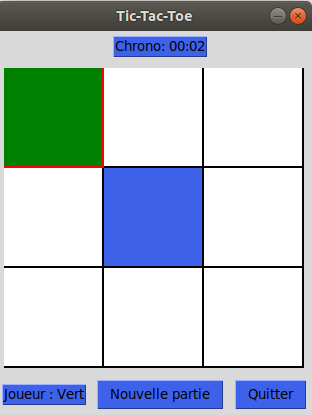
\includegraphics[scale=0.5]{graphiques/morpion.png}
\end{center}

Vous compléterez le squelette de code fourni dans le fichier \texttt{MorpionEleve2021.py},  en insérant des  annotations sous forme de commentaires lorsque les questions ne portent pas sur l'écriture de code Python.


\section{Fixons le cadre}

Précisons les règles du jeu :
{\itshape
\begin{itemize}[label=\ding{43}]
\item Le joueur qui commence est choisi aléatoirement.
\item Chaque joueur identifié par une couleur, joue à tour de rôle, l'un en cliquant sur la case sélectionnée avec le bouton gauche de la souris, l'autre en déplaçant un curseur (cadre rouge autour de la case sélectionnée) avec les flèches du pavé directionnel puis en validant la sélection par un appui sur la touche \texttt{Espace}.  

\item Lorsqu'une case libre a été sélectionnée par un joueur elle prend sa couleur caractéristique, si elle n'est pas libre une fenêtre pop up le signale au joueur.

\item Chaque tour doit s'effectuer en temps limité de 5 seconde, le décompte du temps étant affiché par un chronomètre. Une seconde de pause s'intercale entre deux tours consécutifs.

\item Le jeu s'arrête soit parce qu'un joueur a gagné en  réussissant un alignement de trois cases (horizontal, diagonal ou vertical), soir parce qu'un joueur n'a pas sélectionné de case dans le temps imparti (son adversaire est désigné vainqueur), soit parce que les neuf tours ont été épuisés sans vainqueur (match nul).
\end{itemize}

}

Pour réaliser l'interface graphique, nous utiliserons le module \lstinline+tkinter+ livré avec la distribution standard de \texttt{Python}. Une documentation assez complète sur \lstinline+tkinter+ est disponible sur le web  :

\begin{itemize}[label=\ding{43}]

	\item une documentation en français se trouve sur  \url{http://tkinter.fdex.eu/}.
	
	\item de nombreux exemples sont développés sur \url{http://fsincere.free.fr/isn/python/cours_python_tkinter.php?version=3}
	
\end{itemize}

Par ailleurs, si nous souhaitons afficher  le message de fin de partie dans une fenêtre \texttt{pop-up}, nous aurons besoin du sous-module de \lstinline+tkinter+  nommé \lstinline+tkinter.messagebox+.

Enfin, pour choisir  aléatoirement le joueur qui commence, nous utiliserons le module \lstinline+random+ et pour gérer le temps, nous pourrons employer le module \lstinline+time+.

Commençons donc par éditer avec \texttt{Idle} ou \texttt{Spyder} le fichier  \texttt{MorpionEleve2021.py}. En préambule, on trouve les lignes suivantes pour importer les modules nécessaires, que nous compléterons si besoin en cours de développement :

\begin{lstlisting}
## Modules

from tkinter import *
import  tkinter.messagebox 
import random
import time
\end{lstlisting}

\lstinline+tkinter+ sera le plus utilisé, nous pouvons importer les noms de tous  ses éléments  dans l'espace de nom de notre programme. Les  autres modules ne seront sollicités que ponctuellement et nous  importons juste le module.



\section{Architecture logicielle}


Lorsque le programme sera terminé, il comptera environ 200 lignes, c'est modeste mais suffisant pour l'organiser en trois grandes parties selon \href{https://fr.wikipedia.org/wiki/Mod\%C3\%A8le-vue-contr\%C3\%B4leur}{l'architecture Modèle Vue Contrôleur}.

\begin{center}
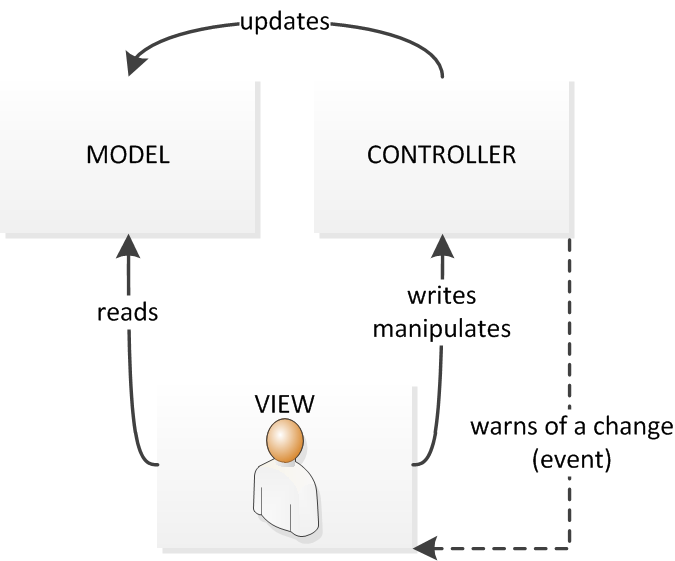
\includegraphics[scale=0.8]{graphiques/ModeleMVC.png}
\end{center}

\begin{itemize}
	\item Le code commence par l'import des modules/bibliothèques nécessaires.
	\item Ensuite vient la partie \textit{Modèle} avec la définition des données et des fonctions permettant de les  manipuler.  On distingue les constantes (couleurs, identifiants des joueurs) et la structure de données principale retournée par la fonction \texttt{initialiser\_grille}  qui est une liste de listes représentant la grille de jeu $3 \times 3$  qui va  enregistrer   les marques déposées par les joueurs. Ces fonctions seront complétées à la fin du projet.

\item La partie \textit{Vue} va rassembler les fonctions permettant de  définir l'interface graphique et des fonctions utilitaires qui leur sont liées. La fonction \verb+interface\_jeu()+ crée puis renvoie les objets graphiques appelés \textit{widgets}.

\item La partie \textit{Contrôleur} réunit les gestionnaires d'événements qui vont s'occuper des interactions entre l'utilisateur et l'interface graphique.
	
\item Enfin le programme principal définit les \textit{widgets} renvoyés par \verb+interface_jeu()+ comme variables globales, fait la liaison avec les gestionnaires d'événements (voir exercice  7) puis la boucle réceptionnaire d'événements. Le nombre d'attributs de l'interface est important, pour organiser ce foisonnement il faudrait utiliser la programmation orientée objet et définir une classe Interface.


\begin{lstlisting}[style=rond]
# Programme principal
if __name__ == "__main__":
    fenetre,  textJoueur, etiquetteJoueur, bouton_quitter, bouton_jouer, textHorloge, horloge,  plateau, case_vers_identifiant, identifiant_vers_case = interface_jeu()
    #Liaisons événements/gestionnaires d'événements
    plateau.bind('<ButtonPress-1>', clic_gauche)
    plateau.bind_all('<KeyPress>', appui_touche)
    #boucle réceptionnaire d'événement 
    fenetre.mainloop()
\end{lstlisting}  

\end{itemize} 
 
 
\begin{exerciceB2}{}

Repérer les parties \textit{Modèle}, \textit{Vue},  \textit{Contrôleur} et le programme principal  dans  \texttt{MorpionEleve2021.py}.

\end{exerciceB2}


\section{Partie Vue : mise en place de l'interface graphique}

{\itshape Dans cette partie, nous allons mettre en place les différents éléments de l'interface graphique. } 


Pour mieux comprendre le fonctionnement du module \texttt{tkinter}, vous travaillerez d'abord avec un autre squelette de code fourni dans le fichier \verb+sandbox_eleve.py+.

\subsection{Fenêtre racine et réceptionnaire d'événements}

\begin{exerciceB2}{}
\begin{minipage}{0.75\linewidth}
L'exécution du programme \verb+sandbox_eleve.py+ produit le résultat ci-contre.

Le code minimal pour afficher  la fenêtre est donné ci-dessous. 

\begin{lstlisting}[numbers=left]
from tkinter import *

#----fenetre principale----
fenetre = Tk()
fenetre.title("Tic-Tac-Toe")
#construire la fenetre à 100 pixels du cote gauche de l'ecran et 150 pixels du cote haut
fenetre.geometry("+100+150")
#interdire la modification de la taille de la fenetre
fenetre.resizable(width=False, height=False)


#----boucle de réception des événements----
#à placer à la fin du programme 
fenetre.mainloop()
\end{lstlisting}
 
\end{minipage}\hfill
\begin{minipage}{0.25\linewidth}
\begin{center}
	
\includegraphics[scale=0.5]{graphiques/tictactoe.png}
\end{center}
\end{minipage}

\begin{enumerate}
	\item Quelles sont les interactions possibles avec la fenêtre ?
	\item Modifier le positionnement de la fenêtre.
	\item Rechercher dans la documentation \url{http://tkinter.fdex.eu/doc/intro.html} le rôle de l'instruction \texttt{fenetre.mainloop()}.
\end{enumerate}
\end{exerciceB2}

\subsection{Widgets}

Nous allons disposer dans la fenêtre racine  \lstinline+fenetre+ des objets graphiques appelés \textbf{widgets}. 

On donne ci-dessous un aperçu de la fenêtre racine contenant  les six widgets.

Ils seront rattachés à \lstinline+fenetre+ par un lien de dépendance et les instructions de construction vont être placées après la création de \lstinline+fenetre+ et juste avant \textbf{la boucle de réception des événements}  \lstinline+fenetre.mainloop()+.

\begin{center}
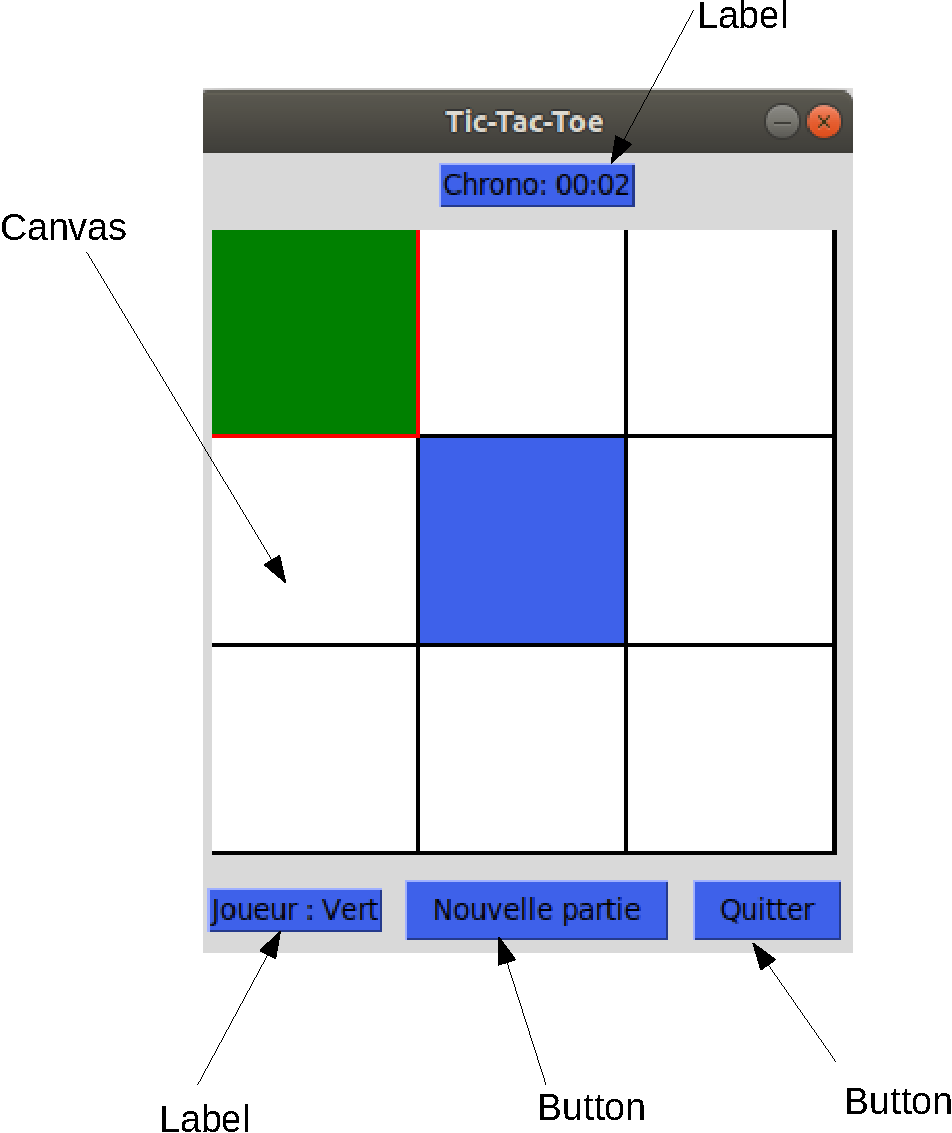
\includegraphics[scale=0.6]{graphiques/widgets-crop.pdf}
\end{center}

\subsubsection{Widget Canvas}

Un \textbf{canevas}  définit une zone rectangulaire qui peut contenir des figures géométriques (rectangles, arcs, ellipses, textes \ldots) ou des images bitmap. 

La documentation se trouve sur la page \url{http://tkinter.fdex.eu/doc/caw.html}.

Nous utilisons un canevas  pour représenter la grille de jeu. Voici les instructions pour le faire apparaître dans la fenêtre. Le canevas définit dans la partie \textit{Vue} l'apparence de la grille (les couleurs des joueurs) alors que la variable \texttt{grille} définie par la fonction \texttt{initialiser\_grille} de la partie \textit{Modèle} contiendra les données de la grille (les marques numériques des joueurs) sur lesquelles s'effectuera la  validation du vainqueur.

\begin{lstlisting}[numbers=left]
#----Canevas----
#il faut diriger les entrées claviers vers le canevas qui n'a pas le focus par défaut
#voir http://tkinter.fdex.eu/doc/focus.html#focus
plateau = Canvas(fenetre, width = COTE_CASE * 3, height = COTE_CASE * 3, bg = 'white', takefocus = 1)
plateau.grid(row = 1, column = 0, columnspan = 3, padx = 5, pady = 5)
\end{lstlisting}

\begin{itemize}[label=\ding{43}]

	\item En ligne 4 on crée le canevas avec le constructeur \lstinline+Canvas+ auquel on passe plusieurs options dont la première, obligatoire, précise qu'il est rattaché à la fenêtre racine \lstinline+fenetre+. On assigne le canevas à une variable \lstinline+plateau+, ce qui permettra de le manipuler   dans la suite du programme.

    \item La ligne 4 ne suffit pas pour afficher le canevas dans la fenêtre. Il faut le placer dans la fenêtre avec la méthode \lstinline+grid+ qui est un \textbf{gestionnaire de placement}. Il existe une méthode similaire  \lstinline+pack+, il ne faut pas mélanger les deux.  \lstinline+grid+  place le widget selon un découpage de la fenêtre en lignes (\lstinline+row+) et colonnes (\lstinline+column+) indexées à partir de $0$.  L'option \lstinline+columnspan+ permet d'étendre le widget sur plusieurs colonnes. Dans notre cas, nous découperons la fenêtre en $3$ colonnes (de $0$ à $2$) et $3$ lignes (de $0$ à $2$).\\    
Les options \lstinline+padx+ et \lstinline+pady+ permettent de définir un espace en pixels autour du widget.


\item Une propriété de widget est accessible en lecture  par la méthode \lstinline+cget+ et en écriture par la méthode \lstinline+configure+. Il existe une syntaxe raccourcie avec l'opérateur \lstinline+[]+ comme pour les dictionnaires.

\begin{lstlisting}
In [14]: plateau['background']
Out[14]: 'white'

In [15]: plateau['background'] = 'red'

In [16]: plateau.cget('background')
Out[16]: 'red'

In [17]: plateau.configure(background = 'white')

In [18]: plateau['bg']    #'bg' est un raccourci pour 'background'
Out[18]: 'white'
\end{lstlisting}

\end{itemize}


\begin{minipage}{0.8\linewidth}
Chaque  case de la grille va être dessinée sur le canevas, muni d'un repère d'origine son coin supérieur gauche avec pour axe des abscisses d'orientation Ouest$\rightarrow$Est le bord supérieur et pour axe des ordonnées  d'orientation Nord$\rightarrow$Sud, le bord gauche. 
\end{minipage}\hfill
\begin{minipage}{0.15\linewidth}
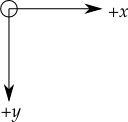
\includegraphics[scale=1]{graphiques/coords.png}
\end{minipage}



Dans le code ci-dessous, la méthode \lstinline+create_rectangle+ permet de représenter la case en ligne d'index $2$ (donc la $3\ieme$ ligne)  et colonne d'index $1$ (donc la $2\ieme$ colonne)  de la grille comme un  rectangle carré de côté \lstinline+COTE_CASE+ pixels, dont le  bord est de couleur \lstinline+COULEUR_BORD_CASE+ avec une épaisseur de $2$ pixels et le fonds de couleur \lstinline+COULEUR_CASE[0]+. Les coordonnées du coin supérieur gauche sont \texttt{(x, y)} et celles du coin inférieur droit sont 
\lstinline*(x + COTE_CASE, y + COTE_CASE)*.

\begin{lstlisting}
x = 1 * COTE_CASE
y = 2 * COTE_CASE
iden = plateau.create_rectangle(x, y , x + COTE_CASE, y + COTE_CASE, outline = COULEUR_BORD_CASE, 
        fill= COULEUR_CASE[0], width=2) 
\end{lstlisting}

\begin{itemize}[label=\ding{43}]

	\item  Attention, les colonnes correspondent aux abscisses et les lignes aux ordonnées. 
	
	\item La méthode \lstinline+create_rectangle+ renvoie l'identifiant unique de l'\textbf{item graphique} (\bcattention le plus petit est $1$). Nous le récupérons dans une variable \lstinline+iden+. Pour retrouver la case, repérée par (ligne, colonne),  à partir de l'identifiant et réciproquement, nous allons créer deux listes de correspondance initialisée avec des valeurs par défaut et nous y stockerons \lstinline+iden+. Nous pourrons ainsi manipuler l'item graphique dans la suite du programme, pour changer son apparence.
\end{itemize}
	
\begin{lstlisting}
case_vers_identifiant = [ [0 for j in range(3)] for i in range(3) ]
identifiant_vers_case = [ (0,0) for k in range(9) ]
#case en ligne 2 et colonne 1 voir code précédent
case_vers_identifiant[2][1] = iden
identifiant_vers_case[iden - 1] = (2, 1)
\end{lstlisting}

	 
%\newpage

\begin{exerciceB2}{}

Dans le fichier \texttt{MorpionEleve2021.py}, compléter   le code de la fonction \verb+interface_jeu+ (à partir de la ligne  195),  pour tracer la grille complète et remplir les listes de correspondance
\lstinline+case_vers_identifiant+ et 

\lstinline+identifiant_vers_case+ avec les identifiants de tous les items graphiques créés.

\begin{minipage}{0.6\linewidth}


On doit obtenir la figure ci-contre sur le canevas.
\end{minipage}\hfill
\begin{minipage}{0.35\linewidth}
\begin{center}
	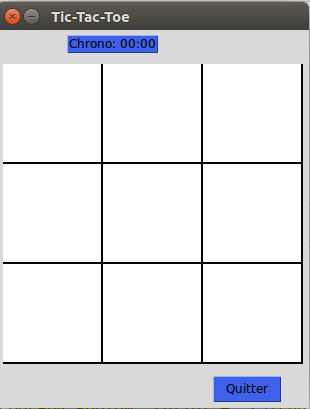
\includegraphics[scale=0.5]{graphiques/morpion-blanc.png}
\end{center}
\end{minipage}
\end{exerciceB2}


\begin{exerciceB2}{}
Compléter la fonction \lstinline+initialiser_plateau+ du fichier \texttt{MorpionEleve2021.py} pour qu'elle initialise 
les neuf rectangles du plateau avec la couleur \lstinline+COULEUR_CASE[0]+. 

On utilisera  la syntaxe :

\lstinline+plateau.itemconfig("ici l'identifiant de la case", fill = "ici la couleur")+.


La documentation se trouve sur \url{http://tkinter.fdex.eu/doc/caw.html#Canvas.itemconfigure}. 

\begin{lstlisting}
def initialiser_plateau(plateau, case_vers_identifiant):
    """Initialise le plateau"""
    for li in range(3):
        for co in range(3):
            "compléter"
\end{lstlisting}

\end{exerciceB2}


\subsubsection{Widgets Label}

Le code ci-dessous permet de créer un widget \lstinline+horloge+ contenant un texte figé pour l'instant. Ce widget est défini dans la fonction \lstinline+interface_jeu+ de \texttt{MorpionEleve2021.py} à partir de la ligne 205.

\begin{lstlisting}[numbers=left]
textHorloge = StringVar()  
textHorloge.set("Chrono: {:02d}:{:02d}".format(0, 0))
horloge = Label(fenetre, textvariable = textHorloge, bg = COULEUR_BOUTON, relief = 'raised')
horloge.grid(row = 0, column = 1, padx = 5, pady = 5)
\end{lstlisting}

\begin{itemize}[label=\ding{43}]
	\item En ligne 3, on crée le widget avec le constructeur \lstinline+Label+ qui sert à afficher une ou plusieurs lignes de texte. On précise obligatoirement que le widget est rattaché à \lstinline+fenetre+, les options suivantes, facultatives, sont  détaillées dans \url{http://tkinter.fdex.eu/doc/labw.html}. Le widget est positionné en ligne 4 du code, avec \lstinline+grid+ : en première ligne (index 0) et deuxième colonne (index 1) de la grille de positionnement.
	\item L'option \lstinline+textvariable+ lie le texte affiché à une variable de contrôle \lstinline+textHorloge+ qui est définie précédemment en ligne 1 avec \lstinline+StringVar+. 
	 \item En ligne 2, le contenu de la  variable de contrôle \lstinline+textHorloge+, de type texte, est modifié avec la méthode \lstinline+set+. On utilise la méthode \lstinline+format+ pour le formatage de la chaîne de caractères. La documentation sur \lstinline+format+ se trouve sur \url{https://docs.python.org/fr/3.5/library/string.html#formatstrings}.
\end{itemize}

Pour animer l'horloge, nous allons utiliser la fonction \lstinline+chronometre+ qui se trouve déjà dans \texttt{MorpionEleve2021.py}.





\begin{lstlisting}[numbers=left]
def chronometre():
    """Fonction récursive qui met à jour l'horloge lors d'un tour"""
    duree = time.time()- debut_tour
    minute, seconde  = divmod(int(duree),  60)
    textHorloge.set("Chrono: {:02d}:{:02d}".format(minute, seconde))
    if duree < TEMPS_MAX:
        fenetre.after(1000, chronometre)
\end{lstlisting}


\begin{itemize}[label=\ding{43}]
	\item En ligne 3, on calcule le temps écoulé, en secondes,  depuis l'origine des temps stockée dans la variable globale \lstinline+debut_tour+, cette dernière sera définie dans la fonction \lstinline+nouvelle_partie+.
	\item En ligne 4, on convertit \lstinline+duree+ en minutes et secondes avec la fonction \lstinline+divmod+ qui retourne le quotient et le reste d'une division euclidienne.
	\item En ligne 5, on modifie la variable de contrôle \lstinline+textHorloge+ avec sa méthode \lstinline+set+. 
	\item En ligne 7, on teste si le temps maximum pour choisir une case (variable  globale \lstinline+TEMPS_MAX+) est dépassé et si ce n'est pas le cas, on appelle de nouveau la fonction \lstinline+chronometre+ après un temps d'attente de $1000$ millisecondes avec la méthode \lstinline+after+ de la fenêtre racine.\\
	La fonction \lstinline+chronometre+  pouvant s'appeler elle-même, c'est une \textbf{fonction récursive}. 
	\end{itemize}
	
\newpage

\begin{exerciceB2}{}
 

\begin{center}
	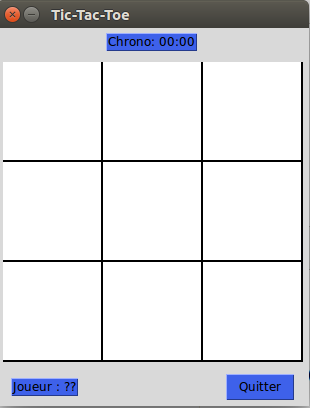
\includegraphics[scale=0.6]{graphiques/morpion-labels.png}
\end{center}	 



Dans la fonction \lstinline+interface_jeu+ de \texttt{MorpionEleve2021.py}, compléter à partir de la ligne 213, le code permettant de créer et positionner dans la fenêtre racine un nouveau  widget de type \lstinline+Label+ :
\begin{itemize}[label=\textbullet]
\item Il doit être stocké dans la variable  \lstinline+etiquetteJoueur+ et placé en \lstinline+row = 2+ et \lstinline+column = 0+.
\item Le texte doit être lié à la variable de contrôle \lstinline+textJoueur = StringVar()+.
\item Ce texte doit indiquer le joueur courant ou "Joueur : ??" si aucune partie n'est en cours. 
\item L'affichage obtenu doit être similaire à celui donné ci-dessus.
\end{itemize}

\end{exerciceB2}

\subsubsection{Widgets Button}

Nous allons placer dans la fenêtre des  widgets de type  \lstinline+Button+ qui sont des boutons d'action.  

La documentation sur les widgets \lstinline+Button+ se trouve sur \url{http://tkinter.fdex.eu/doc/bw.html}.

\begin{lstlisting}[numbers=left]
#----Bouton pour quitter----
bouton_quitter = Button(fenetre, text="Quitter", bg = COULEUR_BOUTON, relief = 'raised',  command = quitter)
bouton_quitter.grid(row = 2, column = 2, padx = 5, pady = 5)
\end{lstlisting}

Détaillons le code ci-dessus qui met en place un bouton qui ferme proprement la fenêtre si on clique dessus. Ce widget est défini dans la fonction \lstinline+interface_jeu+ de \texttt{MorpionEleve2021.py} à partir de la ligne 223.


\begin{itemize}[label=\ding{43}]
	\item En ligne 2, on assigne à la variable \lstinline+bouton_quitter+  un widget \lstinline+Button+ dont l'option \lstinline+command = quitter+ signifie que la fonction \lstinline+quitter+ sera appelée lorsque le bouton recevra un clic gauche. 
	
{\bfseries \bcattention{} Attention, le paramètre de \lstinline+command+ doit être juste le nom de la fonction, sans les parenthèses qui déclenchent son appel. }


	
	Cette fonction est définie en amont et elle permet de fermer la fenêtre proprement.

\begin{lstlisting}[numbers=left]
def quitter():
    """Quitter proprement la fenetre"""
    fenetre.quit()
    fenetre.destroy()
\end{lstlisting}
	
\end{itemize}

\begin{exerciceB2}{}
 
\begin{center}
	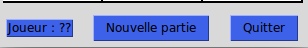
\includegraphics[scale=0.6]{graphiques/morpion-buttons.png}
\end{center}	

\begin{enumerate}

\item Dans la fonction \lstinline+interface_jeu+ de \texttt{MorpionEleve2021.py}, compléter à partir de la ligne 213, lc code permettant de créer et positionner dans la fenêtre racine un nouveau  widget de type \lstinline+Button+ :

\begin{itemize}[label=\textbullet]
\item Il doit être stocké dans la variable  \lstinline+bouton_jouer+ et commander l'appel de la fonction \\ \lstinline+nouvelle_partie+ qui elle même lance la fonction \lstinline+nouveau_tour+.
\item Ce widget doit être placé en ligne d'index \lstinline+row = 2+ et colonne d'index \lstinline+column = 1+ . 
\end{itemize}

\item Le fichier \texttt{MorpionEleve2021.py} contient déjà  les fonctions \lstinline+nouvelle_partie+ et  \lstinline+nouveau_tour+ dont on donne le code ci-dessous.


\begin{enumerate}



	\item Quelle est la portée des variables déclarées avec le mot clef \lstinline+global+ ?
	\item Décrire la séquence d'instruction réalisée par l'appel \lstinline+nouvelle_partie()+.
	\item Quel est le type des variables \lstinline+choix_joueur1+ et \lstinline+choix_joueur2+ ?
	
	Ces variables servent de \textit{drapeaux}  pour indiquer si lors du tour du joueur concerné, une action de sélection de case a déjà été réalisée. Un joueur ne peut en effet sélectionner qu'une seule case lors de son tour.
	
	\item Quel est le point commun entre la fonction \lstinline+nouveau_tour+ et la fonction \lstinline+chronometre+ ?
	
	\item Une partie oppose un joueur 1 et un joueur 2. L'un des deux peut sélectionner une case avec la souris et l'autre avec le clavier en déplaçant un curseur rectangulaire rouge qui entoure la case en haut à gauche de coordonnées $(0,0)$.
	
D'après le code de la fonction \lstinline+nouveau_tour+, quel joueur sélectionne avec le clavier ?

\item Rechercher dans le fichier \lstinline+MorpionEleve2021.py+, le message affiché par l'appel de fonction

 \lstinline+message_fin(vainqueur)+.
\item Décrire la séquence d'instruction réalisée par l'appel \lstinline+nouveau_tour()+.

\end{enumerate}

\begin{lstlisting}[numbers=left]
def nouvelle_partie():
    """Initialise et lance une nouvelle partie"""
    global  vainqueur, joueur, tour, grille, choix_joueur1, choix_joueur2
    grille = initialiser_grille()
    tour = 1
    joueur = random.randint(1, 2)
    textJoueur.set("Joueur : {}".format(COULEUR_JOUEUR[joueur]))
    initialiser_plateau(plateau, case_vers_identifiant)
    vainqueur = 0
    choix_joueur1 = False
    choix_joueur2 = False
    nouveau_tour()
    
def nouveau_tour():
    """Fonction  qui lance un nouveau tour"""
    global vainqueur,joueur, tour, debut_tour, curseur, xcurseur, ycurseur, choix_joueur1, choix_joueur2
    #on positionne les joueurs
    joueur_precedent = joueur
    joueur = adversaire(joueur)
    #mise à jour de l'affichage du joueur
    textJoueur.set("Joueur : {}".format(COULEUR_JOUEUR[joueur]))
    #si le joueur précédent n'a pas cliqué le joueur courant est vainqueur
    #attention à bien mettre des parenthèses autour du or pour changer la priorité par défaut des opérateurs booléens
    if tour >= 2 and (joueur_precedent == JOUEUR_1 and not choix_joueur1 \
    or joueur_precedent == JOUEUR_2 and not choix_joueur2):
        vainqueur = joueur
    #sinon on vérifie si le joueur précédent  a gagné
    elif verifier(grille, joueur_precedent):
        vainqueur = joueur_precedent
    #On affiche le vainqueur sil y en un ou si on a atteint le 10ème tour
    if tour == 10 or vainqueur != 0:
        if joueur == JOUEUR_1:
            plateau.delete(curseur)
        message_fin(vainqueur)
    else: #sinon on commence un nouveau tour
        #pause de 1 seconde avant le changement de joueur
        time.sleep(2)
        #on démarre le chronomètre
        debut_tour = time.time()
        chronometre()
        #on positionne à False les booléens indiquant si le joueur courant a fait son choix
        choix_joueur1 = False
        choix_joueur2 = False
        #pour le joueur 2
        if joueur == JOUEUR_2:
            xcurseur, ycurseur = 0, 0
            curseur = plateau.create_rectangle(xcurseur, ycurseur , xcurseur + COTE_CASE, ycurseur + COTE_CASE,
        outline = 'red',  fill='', width=2)
        elif tour >= 2: #pour le joueur1 à partir du tour 2
            plateau.delete(curseur)
        #on incrémente le compteur de tour pour le tour suivant
        tour = tour + 1
        #on attend TEMPS_MAX secondes (argument en millisecondes) avant de commencer un nouveau tour
        #pendant la durée d'un tour les gestionnaires d'événements gèrent les actions
        fenetre.after(TEMPS_MAX * 1000, nouveau_tour)
\end{lstlisting}

\end{enumerate}

\end{exerciceB2}









\section{Partie contrôleur, les gestionnaires d'événements}


La \textbf{boucle réceptionnaire d'événements} \lstinline+fenetre.mainloop()+ scrute en permanence les \textbf{événements} qui peuvent survenir dans les  widgets.  Un \textbf{événement}  peut être l'appui ou le relâchement d'une touche de clavier, un clic de souris \ldots 

La documentation sur les événements se trouve sur \url{http://tkinter.fdex.eu/doc/event.html}.

Nous avons besoin de gérer deux types d'événements sur le widget \lstinline+plateau+ de type \lstinline+Canvas+.

\begin{itemize}[label=\ding{43}]

	\item un clic gauche sur une case permet de la sélectionner en changeant sa couleur s'il s'agit du tour du joueur autorisé à cliquer, s'il n'a pas déjà sélectionné une case pendant son tour, si la case est libre  et s'il n'y a pas encore de vainqueur.
	
	\item des appuis sur les touches \lstinline+Up+,\lstinline+Down+, \lstinline+Left+, \lstinline+Right+ du pavé directionnel permettent de déplacer le curseur (rectangle rouge) puis de sélectionner une case avec la touche \lstinline+space+ s'il s'agit du tour du joueur autorisé, s'il n'a pas déjà sélectionné une case pendant son tour, si la case est libre  et s'il n'y a pas encore de vainqueur.

\end{itemize}

Un clic gauche de la souris  est l'événement \lstinline+'<ButtonPress-1>'+, alors qu'un appui sur une touche est l'événement \lstinline+'<KeyPress>'+.


Pour chacun de ces événements, le fichier \texttt{MorpionEleve2021.py} contient dans la partie \textit{Contrôleur}, des fonctions qui jouent le rôle de \textbf{gestionnaire d'événement}.

Chaque gestionnaire d'événement \lstinline+clic_gauche+ ou \lstinline+appui_touche+ est attaché à l'événement ciblé par un \textbf{binder} grâce à la méthode \lstinline+bind+ de l'objet canevas stocké dans la variable \lstinline+plateau+. Ces instructions sont placées dans le programme principal, juste   avant l'appel à la boucle réceptionnaire d'événements \lstinline+fenetre.mainloop()+.

\bcattention{} Attention, comme pour le paramètre \lstinline+command+ d'un widget \lstinline+Button+, lors de la liaison, on note juste  le nom du gestionnaire, sans parenthèses.

De plus il faut définir le gestionnaire avant d'établir la liaison.

\begin{lstlisting}[numbers=left]
#Liaisons événements/gestionnaires d'événements
plateau.bind('<ButtonPress-1>', clic_gauche)
plateau.bind_all('<KeyPress>', appui_touche)

fenetre.mainloop()
\end{lstlisting} 

\begin{center}
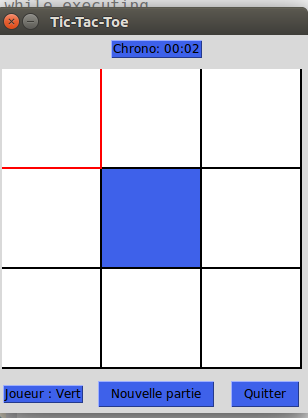
\includegraphics[scale=0.6]{graphiques/morpion-gestionnaire.png}
\end{center}

\begin{exerciceB2}{}

Intéressons-nous au code fourni dans \lstinline+MorpionEleve2021.py+ pour le gestionnaire d'événement \lstinline+'<ButtonPress-1>'+. L'événement capturé est stocké dans le paramètre \lstinline+event+.


\begin{lstlisting}[numbers = left]
def clic_gauche(event):
    """Gestionnaire de clic à gauche, pour le joueur 1"""
    global choix_joueur1
    #clic gauche bloqué si une nouvelle partie n'est pas lancée
    #A MODIFIER pour bloquer le clic s'il y a un vainqueur
    if joueur == JOUEUR_1 and not choix_joueur1 and tour != 0:
        (iden,) = plateau.find_closest(event.x, event.y)
        (lig, col) = identifiant_vers_case[iden - 1]
        if grille[lig][col] != 0:
            showinfo("Erreur", "Case non libre")
        else:
            grille[lig][col] = joueur
            plateau.itemconfig(iden, fill = COULEUR_CASE[joueur])
            choix_joueur1 = True
\end{lstlisting}

\begin{enumerate}
	\item Expliquer les instructions qui permettent de récupérer la case concernée à partir des coordonnées
	du clic.
	\item Quels rôles différents jouent les variables \lstinline+grille+ et \lstinline+plateau+ ?
	\item Pourquoi la variable \lstinline+choix_joueur1+ est-elle déclarée avec le mot clef \lstinline+global+ ?
\end{enumerate}


\end{exerciceB2}



\begin{exerciceB2}{}

Intéressons-nous au code fourni dans \lstinline+MorpionEleve2021.py+ pour le gestionnaire d'événement  \lstinline+'<KeyPress>'+. L'événement capturé est stocké dans le paramètre \lstinline+event+.


\begin{lstlisting}[numbers = left]
def appui_touche(event):
    """Gestionnaire d'appui sur une touche, pour le joueur 2"""
    global choix_joueur2, xcurseur, ycurseur    
    if joueur == JOUEUR_2 and not choix_joueur2 and tour != 0 and vainqueur == 0:
        if event.keysym == 'Left' and xcurseur >= COTE_CASE:
            plateau.coords(curseur, xcurseur - COTE_CASE, ycurseur, xcurseur, ycurseur + COTE_CASE)
            xcurseur, ycurseur = xcurseur - COTE_CASE, ycurseur
        elif event.keysym == 'Up' and ycurseur >= COTE_CASE:
            plateau.coords(curseur, xcurseur, ycurseur - COTE_CASE, xcurseur + COTE_CASE, ycurseur)
            xcurseur, ycurseur = xcurseur, ycurseur - COTE_CASE
        #A MODIFIER : déplacement vers le bas ou la droite
        elif event.keysym == 'space':
            (lig, col) = (ycurseur//COTE_CASE, xcurseur//COTE_CASE)
            if grille[lig][col] == 0:
                iden = case_vers_identifiant[lig][col]
                grille[lig][col] = joueur
                plateau.itemconfig(iden, fill = COULEUR_CASE[joueur])
                choix_joueur2 = True
            else:
                showinfo("Erreur", "Case non libre")
\end{lstlisting}

\begin{enumerate}
	\item Expliquer les modifications des variables \lstinline+xcurseur+ et \lstinline+ycurseur+ lors du déplacement vers la gauche du curseur et la condition nécessaire pour qu'un tel déplacement soit possible.
	
Quelle instruction permet de déplacer le rectangle représentant le curseur dans la fenêtre graphique ?

\item Compléter la fonction \lstinline+appui_touche+ avec des instructions permettent des déplacements vers le haut ou vers le bas.

	
\end{enumerate}


\end{exerciceB2}


\newpage

\section{Partie modèle du jeu et finalisation}

Pour finaliser le jeu, il nous reste à compléter les fonctions de la partie \textit{Modèle} fournie dans \lstinline+MorpionEleve2021.py+.


\begin{exerciceB2}{}



\begin{enumerate}

     \item Compléter la fonction \lstinline+copie(grille)+ pour qu'elle retourne une copie profonde/déréférencée de la grille passée en argument.
     
	  \item Compléter la fonction \lstinline+liste_alignement(grille)+ pour qu'elle  retourne une liste de $8$ listes, représentant chacune les valeurs des cases de l'un des $8$ alignements possibles sur le plateau . En effet, on a $3$ lignes, $3$ colonnes et $2$ diagonales.

\begin{lstlisting}
In [12]: liste_alignement([[0, 0, 2], [0, 1, 0], [2, 0, 1]])
Out[12]: 
[[0, 0, 2],
 [0, 1, 0],
 [2, 0, 1],
 [0, 0, 2],
 [0, 1, 0],
 [2, 0, 1],
 [0, 1, 1],
 [2, 1, 2]]
\end{lstlisting}


\item Compléter la fonction  \lstinline+nb_occurrence(liste, joueur)+ qui prend en argument la liste des valeurs de trois cases alignées sur le plateau et le code d'un joueur ($1$ ou $2$) et qui retourne un couple dont le premier élément est le nombre de cases marquées par le joueur dans l'alignement sélectionné et le deuxième est   le nombre de cases marquées par son adversaire.

\begin{lstlisting}
In [17]: nb_occurrence([1,2,2], 1)
Out[17]: (1, 2)

In [18]: nb_occurrence([1,2,2], 2)
Out[18]: (2, 1)
\end{lstlisting}

\item Compléter la  fonction \lstinline+verifier(grille, joueur)+ pour qu'elle retourne un booléen, \lstinline+True+ si parmi les $8$ alignements possibles, l'un contient $3$ symboles du joueur sélectionné et \lstinline+False+ sinon.

\begin{lstlisting}
In [20]: verifier([[0, 1, 2], [0, 2, 0], [2, 1, 1]], 2)
Out[20]: True
\end{lstlisting}
\end{enumerate}

\end{exerciceB2}




 \end{document}
